%\documentclass{llncs}
\documentclass[final]{IEEEtran}
%%%%%%%%%%%%%%%%%%%%%%
%%%%   PACKAGES   %%%%
%%%%%%%%%%%%%%%%%%%%%%
\usepackage{makeidx}
\usepackage{amsmath}
\usepackage{amssymb}
\usepackage{stmaryrd}
\usepackage{graphicx}
\usepackage{subfigure}
\usepackage{latexsym}
\usepackage{url}
\usepackage{color}
\usepackage{isabelle}
\usepackage{isabellesym}
\usepackage{theorem}
\usepackage{algorithmic}
\usepackage[linesnumbered,ruled,vlined]{algorithm2e}
\usepackage{multicol}
%\usepackage{program}
\usepackage{cases}
\usepackage{enumitem}
%%%%%%%%%%%%%%%%%%%%%%%%%%%%
%For Isabelle code
\newlength{\fminilength}
\newsavebox{\fminibox}
\newenvironment{fmini}[1][\linewidth]
  {\setlength{\fminilength}{#1\fboxsep-2\fboxrule}%
   \vspace{2ex}\noindent\begin{lrbox}{\fminibox}\begin{minipage}{\fminilength}%
   \mbox{ }\hfill\vspace{-2.5ex}}%
  {\end{minipage}\end{lrbox}\vspace{1ex}\hspace{0ex}%
   \framebox{\usebox{\fminibox}}}

\newenvironment{specification}
{\noindent\scriptsize
\tt\begin{fmini}\begin{tabbing}X\=X12345\=XXXX\=XXXX\=XXXX\=XXXX\=XXXX
\=\+\kill} {\end{tabbing}\normalfont\end{fmini}}
\def \twoSpaces {\ \ }
\def \oneSpace {\ }
\def \eqc {\doteq }
\def \andc {\barwedge }
\def \negc {!}
\def \orc {\veebar }
\def \alt {$/\backslash$ }
\def \cat {\symbol{94}}

\def \dbRight {$\backslash\backslash$}
\def \iInv {iInv}
\def \iR {iR}
%%%%%%%%%%%%%%%%%%%%%%%%%%%%

%%%%%%%%%%%%%%%%%%%%%%%%%%%%
%for comments
\newcommand\JP[1]{\textcolor{magenta}{JP: #1}}
\newcommand\lyj[1]{\textcolor{magenta}{lyj: #1}}
\newcommand\cai[1]{\textcolor{blue}{ #1} }
\newcommand\caicomment[1]{\textcolor{red}{comment: #1} }

\setlength{\parskip}{0.6ex}
%%%%%%%%%%%%%%%%%%%%%%%%%%%

%%%%%%%%%%%%%%%%%%%%%%%%%%%
% Additional math operators
%%%%%%%%%%%%%%%%%%%%%%%%%%%

\usepackage[colorlinks,
            linkcolor=black,
            anchorcolor=black,
            citecolor=blue,
            urlcolor=black,
            bookmarks=true
            ]{hyperref}

% Macros for Scientific Word 2.5 documents saved with the LaTeX filter.
%Copyright (C) 1994-95 TCI Software Research, Inc.
\typeout{TCILATEX Macros for Scientific Word 2.5 <22 Dec 95>.}
\typeout{NOTICE:  This macro file is NOT proprietary and may be 
freely copied and distributed.}
%
\makeatletter
%
%%%%%%%%%%%%%%%%%%%%%%
% macros for time
\newcount\@hour\newcount\@minute\chardef\@x10\chardef\@xv60
\def\tcitime{
\def\@time{%
  \@minute\time\@hour\@minute\divide\@hour\@xv
  \ifnum\@hour<\@x 0\fi\the\@hour:%
  \multiply\@hour\@xv\advance\@minute-\@hour
  \ifnum\@minute<\@x 0\fi\the\@minute
  }}%

%%%%%%%%%%%%%%%%%%%%%%
% macro for hyperref
\@ifundefined{hyperref}{\def\hyperref#1#2#3#4{#2\ref{#4}#3}}{}

% macro for external program call
\@ifundefined{qExtProgCall}{\def\qExtProgCall#1#2#3#4#5#6{\relax}}{}
%%%%%%%%%%%%%%%%%%%%%%
%
% macros for graphics
%
\def\FILENAME#1{#1}%
%
\def\QCTOpt[#1]#2{%
  \def\QCTOptB{#1}
  \def\QCTOptA{#2}
}
\def\QCTNOpt#1{%
  \def\QCTOptA{#1}
  \let\QCTOptB\empty
}
\def\Qct{%
  \@ifnextchar[{%
    \QCTOpt}{\QCTNOpt}
}
\def\QCBOpt[#1]#2{%
  \def\QCBOptB{#1}
  \def\QCBOptA{#2}
}
\def\QCBNOpt#1{%
  \def\QCBOptA{#1}
  \let\QCBOptB\empty
}
\def\Qcb{%
  \@ifnextchar[{%
    \QCBOpt}{\QCBNOpt}
}
\def\PrepCapArgs{%
  \ifx\QCBOptA\empty
    \ifx\QCTOptA\empty
      {}%
    \else
      \ifx\QCTOptB\empty
        {\QCTOptA}%
      \else
        [\QCTOptB]{\QCTOptA}%
      \fi
    \fi
  \else
    \ifx\QCBOptA\empty
      {}%
    \else
      \ifx\QCBOptB\empty
        {\QCBOptA}%
      \else
        [\QCBOptB]{\QCBOptA}%
      \fi
    \fi
  \fi
}
\newcount\GRAPHICSTYPE
%\GRAPHICSTYPE 0 is for TurboTeX
%\GRAPHICSTYPE 1 is for DVIWindo (PostScript)
%%%(removed)%\GRAPHICSTYPE 2 is for psfig (PostScript)
\GRAPHICSTYPE=\z@
\def\GRAPHICSPS#1{%
 \ifcase\GRAPHICSTYPE%\GRAPHICSTYPE=0
   \special{ps: #1}%
 \or%\GRAPHICSTYPE=1
   \special{language "PS", include "#1"}%
%%%\or%\GRAPHICSTYPE=2
%%%  #1%
 \fi
}%
%
\def\GRAPHICSHP#1{\special{include #1}}%
%
% \graffile{ body }                                  %#1
%          { contentswidth (scalar)  }               %#2
%          { contentsheight (scalar) }               %#3
%          { vertical shift when in-line (scalar) }  %#4
\def\graffile#1#2#3#4{%
%%% \ifnum\GRAPHICSTYPE=\tw@
%%%  %Following if using psfig
%%%  \@ifundefined{psfig}{\input psfig.tex}{}%
%%%  \psfig{file=#1, height=#3, width=#2}%
%%% \else
  %Following for all others
  % JCS - added BOXTHEFRAME, see below
    \leavevmode
    \raise -#4 \BOXTHEFRAME{%
        \hbox to #2{\raise #3\hbox to #2{\null #1\hfil}}}%
}%
%
% A box for drafts
\def\draftbox#1#2#3#4{%
 \leavevmode\raise -#4 \hbox{%
  \frame{\rlap{\protect\tiny #1}\hbox to #2%
   {\vrule height#3 width\z@ depth\z@\hfil}%
  }%
 }%
}%
%
\newcount\draft
\draft=\z@
\let\nographics=\draft
\newif\ifwasdraft
\wasdraftfalse

%  \GRAPHIC{ body }                                  %#1
%          { draft name }                            %#2
%          { contentswidth (scalar)  }               %#3
%          { contentsheight (scalar) }               %#4
%          { vertical shift when in-line (scalar) }  %#5
\def\GRAPHIC#1#2#3#4#5{%
 \ifnum\draft=\@ne\draftbox{#2}{#3}{#4}{#5}%
  \else\graffile{#1}{#3}{#4}{#5}%
  \fi
 }%
%
\def\addtoLaTeXparams#1{%
    \edef\LaTeXparams{\LaTeXparams #1}}%
%
% JCS -  added a switch BoxFrame that can 
% be set by including X in the frame params.
% If set a box is drawn around the frame.

\newif\ifBoxFrame \BoxFramefalse
\newif\ifOverFrame \OverFramefalse
\newif\ifUnderFrame \UnderFramefalse

\def\BOXTHEFRAME#1{%
   \hbox{%
      \ifBoxFrame
         \frame{#1}%
      \else
         {#1}%
      \fi
   }%
}


\def\doFRAMEparams#1{\BoxFramefalse\OverFramefalse\UnderFramefalse\readFRAMEparams#1\end}%
\def\readFRAMEparams#1{%
 \ifx#1\end%
  \let\next=\relax
  \else
  \ifx#1i\dispkind=\z@\fi
  \ifx#1d\dispkind=\@ne\fi
  \ifx#1f\dispkind=\tw@\fi
  \ifx#1t\addtoLaTeXparams{t}\fi
  \ifx#1b\addtoLaTeXparams{b}\fi
  \ifx#1p\addtoLaTeXparams{p}\fi
  \ifx#1h\addtoLaTeXparams{h}\fi
  \ifx#1X\BoxFrametrue\fi
  \ifx#1O\OverFrametrue\fi
  \ifx#1U\UnderFrametrue\fi
  \ifx#1w
    \ifnum\draft=1\wasdrafttrue\else\wasdraftfalse\fi
    \draft=\@ne
  \fi
  \let\next=\readFRAMEparams
  \fi
 \next
 }%
%
%Macro for In-line graphics object
%   \IFRAME{ contentswidth (scalar)  }               %#1
%          { contentsheight (scalar) }               %#2
%          { vertical shift when in-line (scalar) }  %#3
%          { draft name }                            %#4
%          { body }                                  %#5
%          { caption}                                %#6


\def\IFRAME#1#2#3#4#5#6{%
      \bgroup
      \let\QCTOptA\empty
      \let\QCTOptB\empty
      \let\QCBOptA\empty
      \let\QCBOptB\empty
      #6%
      \parindent=0pt%
      \leftskip=0pt
      \rightskip=0pt
      \setbox0 = \hbox{\QCBOptA}%
      \@tempdima = #1\relax
      \ifOverFrame
          % Do this later
          \typeout{This is not implemented yet}%
          \show\HELP
      \else
         \ifdim\wd0>\@tempdima
            \advance\@tempdima by \@tempdima
            \ifdim\wd0 >\@tempdima
               \textwidth=\@tempdima
               \setbox1 =\vbox{%
                  \noindent\hbox to \@tempdima{\hfill\GRAPHIC{#5}{#4}{#1}{#2}{#3}\hfill}\\%
                  \noindent\hbox to \@tempdima{\parbox[b]{\@tempdima}{\QCBOptA}}%
               }%
               \wd1=\@tempdima
            \else
               \textwidth=\wd0
               \setbox1 =\vbox{%
                 \noindent\hbox to \wd0{\hfill\GRAPHIC{#5}{#4}{#1}{#2}{#3}\hfill}\\%
                 \noindent\hbox{\QCBOptA}%
               }%
               \wd1=\wd0
            \fi
         \else
            %\show\BBB
            \ifdim\wd0>0pt
              \hsize=\@tempdima
              \setbox1 =\vbox{%
                \unskip\GRAPHIC{#5}{#4}{#1}{#2}{0pt}%
                \break
                \unskip\hbox to \@tempdima{\hfill \QCBOptA\hfill}%
              }%
              \wd1=\@tempdima
           \else
              \hsize=\@tempdima
              \setbox1 =\vbox{%
                \unskip\GRAPHIC{#5}{#4}{#1}{#2}{0pt}%
              }%
              \wd1=\@tempdima
           \fi
         \fi
         \@tempdimb=\ht1
         \advance\@tempdimb by \dp1
         \advance\@tempdimb by -#2%
         \advance\@tempdimb by #3%
         \leavevmode
         \raise -\@tempdimb \hbox{\box1}%
      \fi
      \egroup%
}%
%
%Macro for Display graphics object
%   \DFRAME{ contentswidth (scalar)  }               %#1
%          { contentsheight (scalar) }               %#2
%          { draft label }                           %#3
%          { name }                                  %#4
%          { caption}                                %#5
\def\DFRAME#1#2#3#4#5{%
 \begin{center}
     \let\QCTOptA\empty
     \let\QCTOptB\empty
     \let\QCBOptA\empty
     \let\QCBOptB\empty
     \ifOverFrame 
        #5\QCTOptA\par
     \fi
     \GRAPHIC{#4}{#3}{#1}{#2}{\z@}
     \ifUnderFrame 
        \nobreak\par #5\QCBOptA
     \fi
 \end{center}%
 }%
%
%Macro for Floating graphic object
%   \FFRAME{ framedata f|i tbph x F|T }              %#1
%          { contentswidth (scalar)  }               %#2
%          { contentsheight (scalar) }               %#3
%          { caption }                               %#4
%          { label }                                 %#5
%          { draft name }                            %#6
%          { body }                                  %#7
\def\FFRAME#1#2#3#4#5#6#7{%
 \begin{figure}[#1]%
  \let\QCTOptA\empty
  \let\QCTOptB\empty
  \let\QCBOptA\empty
  \let\QCBOptB\empty
  \ifOverFrame
    #4
    \ifx\QCTOptA\empty
    \else
      \ifx\QCTOptB\empty
        \caption{\QCTOptA}%
      \else
        \caption[\QCTOptB]{\QCTOptA}%
      \fi
    \fi
    \ifUnderFrame\else
      \label{#5}%
    \fi
  \else
    \UnderFrametrue%
  \fi
  \begin{center}\GRAPHIC{#7}{#6}{#2}{#3}{\z@}\end{center}%
  \ifUnderFrame
    #4
    \ifx\QCBOptA\empty
      \caption{}%
    \else
      \ifx\QCBOptB\empty
        \caption{\QCBOptA}%
      \else
        \caption[\QCBOptB]{\QCBOptA}%
      \fi
    \fi
    \label{#5}%
  \fi
  \end{figure}%
 }%
%
%
%    \FRAME{ framedata f|i tbph x F|T }              %#1
%          { contentswidth (scalar)  }               %#2
%          { contentsheight (scalar) }               %#3
%          { vertical shift when in-line (scalar) }  %#4
%          { caption }                               %#5
%          { label }                                 %#6
%          { name }                                  %#7
%          { body }                                  %#8
%
%    framedata is a string which can contain the following
%    characters: idftbphxFT
%    Their meaning is as follows:
%             i, d or f : in-line, display, or floating
%             t,b,p,h   : LaTeX floating placement options
%             x         : fit contents box to contents
%             F or T    : Figure or Table. 
%                         Later this can expand
%                         to a more general float class.
%
%
\newcount\dispkind%

\def\makeactives{
  \catcode`\"=\active
  \catcode`\;=\active
  \catcode`\:=\active
  \catcode`\'=\active
  \catcode`\~=\active
}
\bgroup
   \makeactives
   \gdef\activesoff{%
      \def"{\string"}
      \def;{\string;}
      \def:{\string:}
      \def'{\string'}
      \def~{\string~}
      %\bbl@deactivate{"}%
      %\bbl@deactivate{;}%
      %\bbl@deactivate{:}%
      %\bbl@deactivate{'}%
    }
\egroup

\def\FRAME#1#2#3#4#5#6#7#8{%
 \bgroup
 \@ifundefined{bbl@deactivate}{}{\activesoff}
 \ifnum\draft=\@ne
   \wasdrafttrue
 \else
   \wasdraftfalse%
 \fi
 \def\LaTeXparams{}%
 \dispkind=\z@
 \def\LaTeXparams{}%
 \doFRAMEparams{#1}%
 \ifnum\dispkind=\z@\IFRAME{#2}{#3}{#4}{#7}{#8}{#5}\else
  \ifnum\dispkind=\@ne\DFRAME{#2}{#3}{#7}{#8}{#5}\else
   \ifnum\dispkind=\tw@
    \edef\@tempa{\noexpand\FFRAME{\LaTeXparams}}%
    \@tempa{#2}{#3}{#5}{#6}{#7}{#8}%
    \fi
   \fi
  \fi
  \ifwasdraft\draft=1\else\draft=0\fi{}%
  \egroup
 }%
%
% This macro added to let SW gobble a parameter that
% should not be passed on and expanded. 

\def\TEXUX#1{"texux"}

%
% Macros for text attributes:
%
\def\BF#1{{\bf {#1}}}%
\def\NEG#1{\leavevmode\hbox{\rlap{\thinspace/}{$#1$}}}%
%
%%%%%%%%%%%%%%%%%%%%%%%%%%%%%%%%%%%%%%%%%%%%%%%%%%%%%%%%%%%%%%%%%%%%%%%%
%
%
% macros for user - defined functions
\def\func#1{\mathop{\rm #1}}%
\def\limfunc#1{\mathop{\rm #1}}%

%
% miscellaneous 
%\long\def\QQQ#1#2{}%
\long\def\QQQ#1#2{%
     \long\expandafter\def\csname#1\endcsname{#2}}%
%\def\QTP#1{}% JCS - this was changed becuase style editor will define QTP
\@ifundefined{QTP}{\def\QTP#1{}}{}
\@ifundefined{QEXCLUDE}{\def\QEXCLUDE#1{}}{}
%\@ifundefined{Qcb}{\def\Qcb#1{#1}}{}
%\@ifundefined{Qct}{\def\Qct#1{#1}}{}
\@ifundefined{Qlb}{\def\Qlb#1{#1}}{}
\@ifundefined{Qlt}{\def\Qlt#1{#1}}{}
\def\QWE{}%
\long\def\QQA#1#2{}%
%\def\QTR#1#2{{\em #2}}% Always \em!!!
%\def\QTR#1#2{\mbox{\begin{#1}#2\end{#1}}}%cb%%%
\def\QTR#1#2{{\csname#1\endcsname #2}}%(gp) Is this the best?
\long\def\TeXButton#1#2{#2}%
\long\def\QSubDoc#1#2{#2}%
\def\EXPAND#1[#2]#3{}%
\def\NOEXPAND#1[#2]#3{}%
\def\PROTECTED{}%
\def\LaTeXparent#1{}%
\def\ChildStyles#1{}%
\def\ChildDefaults#1{}%
\def\QTagDef#1#2#3{}%
%
% Macros for style editor docs
\@ifundefined{StyleEditBeginDoc}{\def\StyleEditBeginDoc{\relax}}{}
%
% Macros for footnotes
\def\QQfnmark#1{\footnotemark}
\def\QQfntext#1#2{\addtocounter{footnote}{#1}\footnotetext{#2}}
%
% Macros for indexing.
\def\MAKEINDEX{\makeatletter\input gnuindex.sty\makeatother\makeindex}%	
\@ifundefined{INDEX}{\def\INDEX#1#2{}{}}{}%
\@ifundefined{SUBINDEX}{\def\SUBINDEX#1#2#3{}{}{}}{}%
\@ifundefined{initial}%  
   {\def\initial#1{\bigbreak{\raggedright\large\bf #1}\kern 2\p@\penalty3000}}%
   {}%
\@ifundefined{entry}{\def\entry#1#2{\item {#1}, #2}}{}%
\@ifundefined{primary}{\def\primary#1{\item {#1}}}{}%
\@ifundefined{secondary}{\def\secondary#1#2{\subitem {#1}, #2}}{}%
%
%
\@ifundefined{ZZZ}{}{\MAKEINDEX\makeatletter}%
%
% Attempts to avoid problems with other styles
\@ifundefined{abstract}{%
 \def\abstract{%
  \if@twocolumn
   \section*{Abstract (Not appropriate in this style!)}%
   \else \small 
   \begin{center}{\bf Abstract\vspace{-.5em}\vspace{\z@}}\end{center}%
   \quotation 
   \fi
  }%
 }{%
 }%
\@ifundefined{endabstract}{\def\endabstract
  {\if@twocolumn\else\endquotation\fi}}{}%
\@ifundefined{maketitle}{\def\maketitle#1{}}{}%
\@ifundefined{affiliation}{\def\affiliation#1{}}{}%
\@ifundefined{proof}{\def\proof{\noindent{\bfseries Proof. }}}{}%
\@ifundefined{endproof}{\def\endproof{\mbox{\ \rule{.1in}{.1in}}}}{}%
\@ifundefined{newfield}{\def\newfield#1#2{}}{}%
\@ifundefined{chapter}{\def\chapter#1{\par(Chapter head:)#1\par }%
 \newcount\c@chapter}{}%
\@ifundefined{part}{\def\part#1{\par(Part head:)#1\par }}{}%
\@ifundefined{section}{\def\section#1{\par(Section head:)#1\par }}{}%
\@ifundefined{subsection}{\def\subsection#1%
 {\par(Subsection head:)#1\par }}{}%
\@ifundefined{subsubsection}{\def\subsubsection#1%
 {\par(Subsubsection head:)#1\par }}{}%
\@ifundefined{paragraph}{\def\paragraph#1%
 {\par(Subsubsubsection head:)#1\par }}{}%
\@ifundefined{subparagraph}{\def\subparagraph#1%
 {\par(Subsubsubsubsection head:)#1\par }}{}%
%%%%%%%%%%%%%%%%%%%%%%%%%%%%%%%%%%%%%%%%%%%%%%%%%%%%%%%%%%%%%%%%%%%%%%%%
% These symbols are not recognized by LaTeX
\@ifundefined{therefore}{\def\therefore{}}{}%
\@ifundefined{backepsilon}{\def\backepsilon{}}{}%
\@ifundefined{yen}{\def\yen{\hbox{\rm\rlap=Y}}}{}%
\@ifundefined{registered}{%
   \def\registered{\relax\ifmmode{}\r@gistered
                    \else$\m@th\r@gistered$\fi}%
 \def\r@gistered{^{\ooalign
  {\hfil\raise.07ex\hbox{$\scriptstyle\rm\text{R}$}\hfil\crcr
  \mathhexbox20D}}}}{}%
\@ifundefined{Eth}{\def\Eth{}}{}%
\@ifundefined{eth}{\def\eth{}}{}%
\@ifundefined{Thorn}{\def\Thorn{}}{}%
\@ifundefined{thorn}{\def\thorn{}}{}%
% A macro to allow any symbol that requires math to appear in text
\def\TEXTsymbol#1{\mbox{$#1$}}%
\@ifundefined{degree}{\def\degree{{}^{\circ}}}{}%
%
% macros for T3TeX files
\newdimen\theight
\def\Column{%
 \vadjust{\setbox\z@=\hbox{\scriptsize\quad\quad tcol}%
  \theight=\ht\z@\advance\theight by \dp\z@\advance\theight by \lineskip
  \kern -\theight \vbox to \theight{%
   \rightline{\rlap{\box\z@}}%
   \vss
   }%
  }%
 }%
%
\def\qed{%
 \ifhmode\unskip\nobreak\fi\ifmmode\ifinner\else\hskip5\p@\fi\fi
 \hbox{\hskip5\p@\vrule width4\p@ height6\p@ depth1.5\p@\hskip\p@}%
 }%
%
\def\cents{\hbox{\rm\rlap/c}}%
\def\miss{\hbox{\vrule height2\p@ width 2\p@ depth\z@}}%
%\def\miss{\hbox{.}}%        %another possibility 
%
\def\vvert{\Vert}%           %always translated to \left| or \right|
%
\def\tcol#1{{\baselineskip=6\p@ \vcenter{#1}} \Column}  %
%
\def\dB{\hbox{{}}}%                 %dummy entry in column 
\def\mB#1{\hbox{$#1$}}%             %column entry
\def\nB#1{\hbox{#1}}%               %column entry (not math)
%
%\newcount\notenumber
%\def\clearnotenumber{\notenumber=0}
%\def\note{\global\advance\notenumber by 1
% \footnote{$^{\the\notenumber}$}}
%\def\note{\global\advance\notenumber by 1
\def\note{$^{\dag}}%
%
%

\def\newfmtname{LaTeX2e}
\def\chkcompat{%
   \if@compatibility
   \else
     \usepackage{latexsym}
   \fi
}

\ifx\fmtname\newfmtname
  \DeclareOldFontCommand{\rm}{\normalfont\rmfamily}{\mathrm}
  \DeclareOldFontCommand{\sf}{\normalfont\sffamily}{\mathsf}
  \DeclareOldFontCommand{\tt}{\normalfont\ttfamily}{\mathtt}
  \DeclareOldFontCommand{\bf}{\normalfont\bfseries}{\mathbf}
  \DeclareOldFontCommand{\it}{\normalfont\itshape}{\mathit}
  \DeclareOldFontCommand{\sl}{\normalfont\slshape}{\@nomath\sl}
  \DeclareOldFontCommand{\sc}{\normalfont\scshape}{\@nomath\sc}
  \chkcompat
\fi

%
% Greek bold macros
% Redefine all of the math symbols 
% which might be bolded	 - there are 
% probably others to add to this list

\def\alpha{\Greekmath 010B }%
\def\beta{\Greekmath 010C }%
\def\gamma{\Greekmath 010D }%
\def\delta{\Greekmath 010E }%
\def\epsilon{\Greekmath 010F }%
\def\zeta{\Greekmath 0110 }%
\def\eta{\Greekmath 0111 }%
\def\theta{\Greekmath 0112 }%
\def\iota{\Greekmath 0113 }%
\def\kappa{\Greekmath 0114 }%
\def\lambda{\Greekmath 0115 }%
\def\mu{\Greekmath 0116 }%
\def\nu{\Greekmath 0117 }%
\def\xi{\Greekmath 0118 }%
\def\pi{\Greekmath 0119 }%
\def\rho{\Greekmath 011A }%
\def\sigma{\Greekmath 011B }%
\def\tau{\Greekmath 011C }%
\def\upsilon{\Greekmath 011D }%
\def\phi{\Greekmath 011E }%
\def\chi{\Greekmath 011F }%
\def\psi{\Greekmath 0120 }%
\def\omega{\Greekmath 0121 }%
\def\varepsilon{\Greekmath 0122 }%
\def\vartheta{\Greekmath 0123 }%
\def\varpi{\Greekmath 0124 }%
\def\varrho{\Greekmath 0125 }%
\def\varsigma{\Greekmath 0126 }%
\def\varphi{\Greekmath 0127 }%

\def\nabla{\Greekmath 0272 }
\def\FindBoldGroup{%
   {\setbox0=\hbox{$\mathbf{x\global\edef\theboldgroup{\the\mathgroup}}$}}%
}

\def\Greekmath#1#2#3#4{%
    \if@compatibility
        \ifnum\mathgroup=\symbold
           \mathchoice{\mbox{\boldmath$\displaystyle\mathchar"#1#2#3#4$}}%
                      {\mbox{\boldmath$\textstyle\mathchar"#1#2#3#4$}}%
                      {\mbox{\boldmath$\scriptstyle\mathchar"#1#2#3#4$}}%
                      {\mbox{\boldmath$\scriptscriptstyle\mathchar"#1#2#3#4$}}%
        \else
           \mathchar"#1#2#3#4% 
        \fi 
    \else 
        \FindBoldGroup
        \ifnum\mathgroup=\theboldgroup % For 2e
           \mathchoice{\mbox{\boldmath$\displaystyle\mathchar"#1#2#3#4$}}%
                      {\mbox{\boldmath$\textstyle\mathchar"#1#2#3#4$}}%
                      {\mbox{\boldmath$\scriptstyle\mathchar"#1#2#3#4$}}%
                      {\mbox{\boldmath$\scriptscriptstyle\mathchar"#1#2#3#4$}}%
        \else
           \mathchar"#1#2#3#4% 
        \fi     	    
	  \fi}

\newif\ifGreekBold  \GreekBoldfalse
\let\SAVEPBF=\pbf
\def\pbf{\GreekBoldtrue\SAVEPBF}%
%

\@ifundefined{theorem}{\newtheorem{theorem}{Theorem}}{}
\@ifundefined{lemma}{\newtheorem{lemma}[theorem]{Lemma}}{}
\@ifundefined{corollary}{\newtheorem{corollary}[theorem]{Corollary}}{}
\@ifundefined{conjecture}{\newtheorem{conjecture}[theorem]{Conjecture}}{}
\@ifundefined{proposition}{\newtheorem{proposition}[theorem]{Proposition}}{}
\@ifundefined{axiom}{\newtheorem{axiom}{Axiom}}{}
\@ifundefined{remark}{\newtheorem{remark}{Remark}}{}
\@ifundefined{example}{\newtheorem{example}{Example}}{}
\@ifundefined{exercise}{\newtheorem{exercise}{Exercise}}{}
\@ifundefined{definition}{\newtheorem{definition}{Definition}}{}


\@ifundefined{mathletters}{%
  %\def\theequation{\arabic{equation}}
  \newcounter{equationnumber}  
  \def\mathletters{%
     \addtocounter{equation}{1}
     \edef\@currentlabel{\theequation}%
     \setcounter{equationnumber}{\c@equation}
     \setcounter{equation}{0}%
     \edef\theequation{\@currentlabel\noexpand\alph{equation}}%
  }
  \def\endmathletters{%
     \setcounter{equation}{\value{equationnumber}}%
  }
}{}

%Logos
\@ifundefined{BibTeX}{%
    \def\BibTeX{{\rm B\kern-.05em{\sc i\kern-.025em b}\kern-.08em
                 T\kern-.1667em\lower.7ex\hbox{E}\kern-.125emX}}}{}%
\@ifundefined{AmS}%
    {\def\AmS{{\protect\usefont{OMS}{cmsy}{m}{n}%
                A\kern-.1667em\lower.5ex\hbox{M}\kern-.125emS}}}{}%
\@ifundefined{AmSTeX}{\def\AmSTeX{\protect\AmS-\protect\TeX\@}}{}%
%

%%%%%%%%%%%%%%%%%%%%%%%%%%%%%%%%%%%%%%%%%%%%%%%%%%%%%%%%%%%%%%%%%%%%%%%
% NOTE: The rest of this file is read only if amstex has not been
% loaded.  This section is used to define amstex constructs in the
% event they have not been defined.
%
%
\ifx\ds@amstex\relax
   \message{amstex already loaded}\makeatother\endinput% 2.09 compatability
\else
   \@ifpackageloaded{amstex}%
      {\message{amstex already loaded}\makeatother\endinput}
      {}
   \@ifpackageloaded{amsgen}%
      {\message{amsgen already loaded}\makeatother\endinput}
      {}
\fi
%%%%%%%%%%%%%%%%%%%%%%%%%%%%%%%%%%%%%%%%%%%%%%%%%%%%%%%%%%%%%%%%%%%%%%%%
%%
%
%
%  Macros to define some AMS LaTeX constructs when 
%  AMS LaTeX has not been loaded
% 
% These macros are copied from the AMS-TeX package for doing
% multiple integrals.
%
\let\DOTSI\relax
\def\RIfM@{\relax\ifmmode}%
\def\FN@{\futurelet\next}%
\newcount\intno@
\def\iint{\DOTSI\intno@\tw@\FN@\ints@}%
\def\iiint{\DOTSI\intno@\thr@@\FN@\ints@}%
\def\iiiint{\DOTSI\intno@4 \FN@\ints@}%
\def\idotsint{\DOTSI\intno@\z@\FN@\ints@}%
\def\ints@{\findlimits@\ints@@}%
\newif\iflimtoken@
\newif\iflimits@
\def\findlimits@{\limtoken@true\ifx\next\limits\limits@true
 \else\ifx\next\nolimits\limits@false\else
 \limtoken@false\ifx\ilimits@\nolimits\limits@false\else
 \ifinner\limits@false\else\limits@true\fi\fi\fi\fi}%
\def\multint@{\int\ifnum\intno@=\z@\intdots@                          %1
 \else\intkern@\fi                                                    %2
 \ifnum\intno@>\tw@\int\intkern@\fi                                   %3
 \ifnum\intno@>\thr@@\int\intkern@\fi                                 %4
 \int}%                                                               %5
\def\multintlimits@{\intop\ifnum\intno@=\z@\intdots@\else\intkern@\fi
 \ifnum\intno@>\tw@\intop\intkern@\fi
 \ifnum\intno@>\thr@@\intop\intkern@\fi\intop}%
\def\intic@{%
    \mathchoice{\hskip.5em}{\hskip.4em}{\hskip.4em}{\hskip.4em}}%
\def\negintic@{\mathchoice
 {\hskip-.5em}{\hskip-.4em}{\hskip-.4em}{\hskip-.4em}}%
\def\ints@@{\iflimtoken@                                              %1
 \def\ints@@@{\iflimits@\negintic@
   \mathop{\intic@\multintlimits@}\limits                             %2
  \else\multint@\nolimits\fi                                          %3
  \eat@}%                                                             %4
 \else                                                                %5
 \def\ints@@@{\iflimits@\negintic@
  \mathop{\intic@\multintlimits@}\limits\else
  \multint@\nolimits\fi}\fi\ints@@@}%
\def\intkern@{\mathchoice{\!\!\!}{\!\!}{\!\!}{\!\!}}%
\def\plaincdots@{\mathinner{\cdotp\cdotp\cdotp}}%
\def\intdots@{\mathchoice{\plaincdots@}%
 {{\cdotp}\mkern1.5mu{\cdotp}\mkern1.5mu{\cdotp}}%
 {{\cdotp}\mkern1mu{\cdotp}\mkern1mu{\cdotp}}%
 {{\cdotp}\mkern1mu{\cdotp}\mkern1mu{\cdotp}}}%
%
%
%  These macros are for doing the AMS \text{} construct
%
\def\RIfM@{\relax\protect\ifmmode}
\def\text{\RIfM@\expandafter\text@\else\expandafter\mbox\fi}
\let\nfss@text\text
\def\text@#1{\mathchoice
   {\textdef@\displaystyle\f@size{#1}}%
   {\textdef@\textstyle\tf@size{\firstchoice@false #1}}%
   {\textdef@\textstyle\sf@size{\firstchoice@false #1}}%
   {\textdef@\textstyle \ssf@size{\firstchoice@false #1}}%
   \glb@settings}

\def\textdef@#1#2#3{\hbox{{%
                    \everymath{#1}%
                    \let\f@size#2\selectfont
                    #3}}}
\newif\iffirstchoice@
\firstchoice@true
%
%    Old Scheme for \text
%
%\def\rmfam{\z@}%
%\newif\iffirstchoice@
%\firstchoice@true
%\def\textfonti{\the\textfont\@ne}%
%\def\textfontii{\the\textfont\tw@}%
%\def\text{\RIfM@\expandafter\text@\else\expandafter\text@@\fi}%
%\def\text@@#1{\leavevmode\hbox{#1}}%
%\def\text@#1{\mathchoice
% {\hbox{\everymath{\displaystyle}\def\textfonti{\the\textfont\@ne}%
%  \def\textfontii{\the\textfont\tw@}\textdef@@ T#1}}%
% {\hbox{\firstchoice@false
%  \everymath{\textstyle}\def\textfonti{\the\textfont\@ne}%
%  \def\textfontii{\the\textfont\tw@}\textdef@@ T#1}}%
% {\hbox{\firstchoice@false
%  \everymath{\scriptstyle}\def\textfonti{\the\scriptfont\@ne}%
%  \def\textfontii{\the\scriptfont\tw@}\textdef@@ S\rm#1}}%
% {\hbox{\firstchoice@false
%  \everymath{\scriptscriptstyle}\def\textfonti
%  {\the\scriptscriptfont\@ne}%
%  \def\textfontii{\the\scriptscriptfont\tw@}\textdef@@ s\rm#1}}}%
%\def\textdef@@#1{\textdef@#1\rm\textdef@#1\bf\textdef@#1\sl
%    \textdef@#1\it}%
%\def\DN@{\def\next@}%
%\def\eat@#1{}%
%\def\textdef@#1#2{%
% \DN@{\csname\expandafter\eat@\string#2fam\endcsname}%
% \if S#1\edef#2{\the\scriptfont\next@\relax}%
% \else\if s#1\edef#2{\the\scriptscriptfont\next@\relax}%
% \else\edef#2{\the\textfont\next@\relax}\fi\fi}%
%
%
%These are the AMS constructs for multiline limits.
%
\def\Let@{\relax\iffalse{\fi\let\\=\cr\iffalse}\fi}%
\def\vspace@{\def\vspace##1{\crcr\noalign{\vskip##1\relax}}}%
\def\multilimits@{\bgroup\vspace@\Let@
 \baselineskip\fontdimen10 \scriptfont\tw@
 \advance\baselineskip\fontdimen12 \scriptfont\tw@
 \lineskip\thr@@\fontdimen8 \scriptfont\thr@@
 \lineskiplimit\lineskip
 \vbox\bgroup\ialign\bgroup\hfil$\m@th\scriptstyle{##}$\hfil\crcr}%
\def\Sb{_\multilimits@}%
\def\endSb{\crcr\egroup\egroup\egroup}%
\def\Sp{^\multilimits@}%
\let\endSp\endSb
%
%
%These are AMS constructs for horizontal arrows
%
\newdimen\ex@
\ex@.2326ex
\def\rightarrowfill@#1{$#1\m@th\mathord-\mkern-6mu\cleaders
 \hbox{$#1\mkern-2mu\mathord-\mkern-2mu$}\hfill
 \mkern-6mu\mathord\rightarrow$}%
\def\leftarrowfill@#1{$#1\m@th\mathord\leftarrow\mkern-6mu\cleaders
 \hbox{$#1\mkern-2mu\mathord-\mkern-2mu$}\hfill\mkern-6mu\mathord-$}%
\def\leftrightarrowfill@#1{$#1\m@th\mathord\leftarrow
\mkern-6mu\cleaders
 \hbox{$#1\mkern-2mu\mathord-\mkern-2mu$}\hfill
 \mkern-6mu\mathord\rightarrow$}%
\def\overrightarrow{\mathpalette\overrightarrow@}%
\def\overrightarrow@#1#2{\vbox{\ialign{##\crcr\rightarrowfill@#1\crcr
 \noalign{\kern-\ex@\nointerlineskip}$\m@th\hfil#1#2\hfil$\crcr}}}%
\let\overarrow\overrightarrow
\def\overleftarrow{\mathpalette\overleftarrow@}%
\def\overleftarrow@#1#2{\vbox{\ialign{##\crcr\leftarrowfill@#1\crcr
 \noalign{\kern-\ex@\nointerlineskip}$\m@th\hfil#1#2\hfil$\crcr}}}%
\def\overleftrightarrow{\mathpalette\overleftrightarrow@}%
\def\overleftrightarrow@#1#2{\vbox{\ialign{##\crcr
   \leftrightarrowfill@#1\crcr
 \noalign{\kern-\ex@\nointerlineskip}$\m@th\hfil#1#2\hfil$\crcr}}}%
\def\underrightarrow{\mathpalette\underrightarrow@}%
\def\underrightarrow@#1#2{\vtop{\ialign{##\crcr$\m@th\hfil#1#2\hfil
  $\crcr\noalign{\nointerlineskip}\rightarrowfill@#1\crcr}}}%
\let\underarrow\underrightarrow
\def\underleftarrow{\mathpalette\underleftarrow@}%
\def\underleftarrow@#1#2{\vtop{\ialign{##\crcr$\m@th\hfil#1#2\hfil
  $\crcr\noalign{\nointerlineskip}\leftarrowfill@#1\crcr}}}%
\def\underleftrightarrow{\mathpalette\underleftrightarrow@}%
\def\underleftrightarrow@#1#2{\vtop{\ialign{##\crcr$\m@th
  \hfil#1#2\hfil$\crcr
 \noalign{\nointerlineskip}\leftrightarrowfill@#1\crcr}}}%
%%%%%%%%%%%%%%%%%%%%%

% 94.0815 by Jon:

\def\qopnamewl@#1{\mathop{\operator@font#1}\nlimits@}
\let\nlimits@\displaylimits
\def\setboxz@h{\setbox\z@\hbox}


\def\varlim@#1#2{\mathop{\vtop{\ialign{##\crcr
 \hfil$#1\m@th\operator@font lim$\hfil\crcr
 \noalign{\nointerlineskip}#2#1\crcr
 \noalign{\nointerlineskip\kern-\ex@}\crcr}}}}

 \def\rightarrowfill@#1{\m@th\setboxz@h{$#1-$}\ht\z@\z@
  $#1\copy\z@\mkern-6mu\cleaders
  \hbox{$#1\mkern-2mu\box\z@\mkern-2mu$}\hfill
  \mkern-6mu\mathord\rightarrow$}
\def\leftarrowfill@#1{\m@th\setboxz@h{$#1-$}\ht\z@\z@
  $#1\mathord\leftarrow\mkern-6mu\cleaders
  \hbox{$#1\mkern-2mu\copy\z@\mkern-2mu$}\hfill
  \mkern-6mu\box\z@$}


\def\projlim{\qopnamewl@{proj\,lim}}
\def\injlim{\qopnamewl@{inj\,lim}}
\def\varinjlim{\mathpalette\varlim@\rightarrowfill@}
\def\varprojlim{\mathpalette\varlim@\leftarrowfill@}
\def\varliminf{\mathpalette\varliminf@{}}
\def\varliminf@#1{\mathop{\underline{\vrule\@depth.2\ex@\@width\z@
   \hbox{$#1\m@th\operator@font lim$}}}}
\def\varlimsup{\mathpalette\varlimsup@{}}
\def\varlimsup@#1{\mathop{\overline
  {\hbox{$#1\m@th\operator@font lim$}}}}

%
%%%%%%%%%%%%%%%%%%%%%%%%%%%%%%%%%%%%%%%%%%%%%%%%%%%%%%%%%%%%%%%%%%%%%
%
\def\tfrac#1#2{{\textstyle {#1 \over #2}}}%
\def\dfrac#1#2{{\displaystyle {#1 \over #2}}}%
\def\binom#1#2{{#1 \choose #2}}%
\def\tbinom#1#2{{\textstyle {#1 \choose #2}}}%
\def\dbinom#1#2{{\displaystyle {#1 \choose #2}}}%
\def\QATOP#1#2{{#1 \atop #2}}%
\def\QTATOP#1#2{{\textstyle {#1 \atop #2}}}%
\def\QDATOP#1#2{{\displaystyle {#1 \atop #2}}}%
\def\QABOVE#1#2#3{{#2 \above#1 #3}}%
\def\QTABOVE#1#2#3{{\textstyle {#2 \above#1 #3}}}%
\def\QDABOVE#1#2#3{{\displaystyle {#2 \above#1 #3}}}%
\def\QOVERD#1#2#3#4{{#3 \overwithdelims#1#2 #4}}%
\def\QTOVERD#1#2#3#4{{\textstyle {#3 \overwithdelims#1#2 #4}}}%
\def\QDOVERD#1#2#3#4{{\displaystyle {#3 \overwithdelims#1#2 #4}}}%
\def\QATOPD#1#2#3#4{{#3 \atopwithdelims#1#2 #4}}%
\def\QTATOPD#1#2#3#4{{\textstyle {#3 \atopwithdelims#1#2 #4}}}%
\def\QDATOPD#1#2#3#4{{\displaystyle {#3 \atopwithdelims#1#2 #4}}}%
\def\QABOVED#1#2#3#4#5{{#4 \abovewithdelims#1#2#3 #5}}%
\def\QTABOVED#1#2#3#4#5{{\textstyle 
   {#4 \abovewithdelims#1#2#3 #5}}}%
\def\QDABOVED#1#2#3#4#5{{\displaystyle 
   {#4 \abovewithdelims#1#2#3 #5}}}%
%
% Macros for text size operators:

%JCS - added braces and \mathop around \displaystyle\int, etc.
%
\def\tint{\mathop{\textstyle \int}}%
\def\tiint{\mathop{\textstyle \iint }}%
\def\tiiint{\mathop{\textstyle \iiint }}%
\def\tiiiint{\mathop{\textstyle \iiiint }}%
\def\tidotsint{\mathop{\textstyle \idotsint }}%
\def\toint{\mathop{\textstyle \oint}}%
\def\tsum{\mathop{\textstyle \sum }}%
\def\tprod{\mathop{\textstyle \prod }}%
\def\tbigcap{\mathop{\textstyle \bigcap }}%
\def\tbigwedge{\mathop{\textstyle \bigwedge }}%
\def\tbigoplus{\mathop{\textstyle \bigoplus }}%
\def\tbigodot{\mathop{\textstyle \bigodot }}%
\def\tbigsqcup{\mathop{\textstyle \bigsqcup }}%
\def\tcoprod{\mathop{\textstyle \coprod }}%
\def\tbigcup{\mathop{\textstyle \bigcup }}%
\def\tbigvee{\mathop{\textstyle \bigvee }}%
\def\tbigotimes{\mathop{\textstyle \bigotimes }}%
\def\tbiguplus{\mathop{\textstyle \biguplus }}%
%
%
%Macros for display size operators:
%

\def\dint{\mathop{\displaystyle \int}}%
\def\diint{\mathop{\displaystyle \iint }}%
\def\diiint{\mathop{\displaystyle \iiint }}%
\def\diiiint{\mathop{\displaystyle \iiiint }}%
\def\didotsint{\mathop{\displaystyle \idotsint }}%
\def\doint{\mathop{\displaystyle \oint}}%
\def\dsum{\mathop{\displaystyle \sum }}%
\def\dprod{\mathop{\displaystyle \prod }}%
\def\dbigcap{\mathop{\displaystyle \bigcap }}%
\def\dbigwedge{\mathop{\displaystyle \bigwedge }}%
\def\dbigoplus{\mathop{\displaystyle \bigoplus }}%
\def\dbigodot{\mathop{\displaystyle \bigodot }}%
\def\dbigsqcup{\mathop{\displaystyle \bigsqcup }}%
\def\dcoprod{\mathop{\displaystyle \coprod }}%
\def\dbigcup{\mathop{\displaystyle \bigcup }}%
\def\dbigvee{\mathop{\displaystyle \bigvee }}%
\def\dbigotimes{\mathop{\displaystyle \bigotimes }}%
\def\dbiguplus{\mathop{\displaystyle \biguplus }}%
%
%Companion to stackrel
\def\stackunder#1#2{\mathrel{\mathop{#2}\limits_{#1}}}%
%
%
% These are AMS environments that will be defined to
% be verbatims if amstex has not actually been 
% loaded
%
%
\begingroup \catcode `|=0 \catcode `[= 1
\catcode`]=2 \catcode `\{=12 \catcode `\}=12
\catcode`\\=12 
|gdef|@alignverbatim#1\end{align}[#1|end[align]]
|gdef|@salignverbatim#1\end{align*}[#1|end[align*]]

|gdef|@alignatverbatim#1\end{alignat}[#1|end[alignat]]
|gdef|@salignatverbatim#1\end{alignat*}[#1|end[alignat*]]

|gdef|@xalignatverbatim#1\end{xalignat}[#1|end[xalignat]]
|gdef|@sxalignatverbatim#1\end{xalignat*}[#1|end[xalignat*]]

|gdef|@gatherverbatim#1\end{gather}[#1|end[gather]]
|gdef|@sgatherverbatim#1\end{gather*}[#1|end[gather*]]

|gdef|@gatherverbatim#1\end{gather}[#1|end[gather]]
|gdef|@sgatherverbatim#1\end{gather*}[#1|end[gather*]]


|gdef|@multilineverbatim#1\end{multiline}[#1|end[multiline]]
|gdef|@smultilineverbatim#1\end{multiline*}[#1|end[multiline*]]

|gdef|@arraxverbatim#1\end{arrax}[#1|end[arrax]]
|gdef|@sarraxverbatim#1\end{arrax*}[#1|end[arrax*]]

|gdef|@tabulaxverbatim#1\end{tabulax}[#1|end[tabulax]]
|gdef|@stabulaxverbatim#1\end{tabulax*}[#1|end[tabulax*]]


|endgroup
  

  
\def\align{\@verbatim \frenchspacing\@vobeyspaces \@alignverbatim
You are using the "align" environment in a style in which it is not defined.}
\let\endalign=\endtrivlist
 
\@namedef{align*}{\@verbatim\@salignverbatim
You are using the "align*" environment in a style in which it is not defined.}
\expandafter\let\csname endalign*\endcsname =\endtrivlist




\def\alignat{\@verbatim \frenchspacing\@vobeyspaces \@alignatverbatim
You are using the "alignat" environment in a style in which it is not defined.}
\let\endalignat=\endtrivlist
 
\@namedef{alignat*}{\@verbatim\@salignatverbatim
You are using the "alignat*" environment in a style in which it is not defined.}
\expandafter\let\csname endalignat*\endcsname =\endtrivlist




\def\xalignat{\@verbatim \frenchspacing\@vobeyspaces \@xalignatverbatim
You are using the "xalignat" environment in a style in which it is not defined.}
\let\endxalignat=\endtrivlist
 
\@namedef{xalignat*}{\@verbatim\@sxalignatverbatim
You are using the "xalignat*" environment in a style in which it is not defined.}
\expandafter\let\csname endxalignat*\endcsname =\endtrivlist




\def\gather{\@verbatim \frenchspacing\@vobeyspaces \@gatherverbatim
You are using the "gather" environment in a style in which it is not defined.}
\let\endgather=\endtrivlist
 
\@namedef{gather*}{\@verbatim\@sgatherverbatim
You are using the "gather*" environment in a style in which it is not defined.}
\expandafter\let\csname endgather*\endcsname =\endtrivlist


\def\multiline{\@verbatim \frenchspacing\@vobeyspaces \@multilineverbatim
You are using the "multiline" environment in a style in which it is not defined.}
\let\endmultiline=\endtrivlist
 
\@namedef{multiline*}{\@verbatim\@smultilineverbatim
You are using the "multiline*" environment in a style in which it is not defined.}
\expandafter\let\csname endmultiline*\endcsname =\endtrivlist


\def\arrax{\@verbatim \frenchspacing\@vobeyspaces \@arraxverbatim
You are using a type of "array" construct that is only allowed in AmS-LaTeX.}
\let\endarrax=\endtrivlist

\def\tabulax{\@verbatim \frenchspacing\@vobeyspaces \@tabulaxverbatim
You are using a type of "tabular" construct that is only allowed in AmS-LaTeX.}
\let\endtabulax=\endtrivlist

 
\@namedef{arrax*}{\@verbatim\@sarraxverbatim
You are using a type of "array*" construct that is only allowed in AmS-LaTeX.}
\expandafter\let\csname endarrax*\endcsname =\endtrivlist

\@namedef{tabulax*}{\@verbatim\@stabulaxverbatim
You are using a type of "tabular*" construct that is only allowed in AmS-LaTeX.}
\expandafter\let\csname endtabulax*\endcsname =\endtrivlist

% macro to simulate ams tag construct


% This macro is a fix to eqnarray
\def\@@eqncr{\let\@tempa\relax
    \ifcase\@eqcnt \def\@tempa{& & &}\or \def\@tempa{& &}%
      \else \def\@tempa{&}\fi
     \@tempa
     \if@eqnsw
        \iftag@
           \@taggnum
        \else
           \@eqnnum\stepcounter{equation}%
        \fi
     \fi
     \global\tag@false
     \global\@eqnswtrue
     \global\@eqcnt\z@\cr}


% This macro is a fix to the equation environment
 \def\endequation{%
     \ifmmode\ifinner % FLEQN hack
      \iftag@
        \addtocounter{equation}{-1} % undo the increment made in the begin part
        $\hfil
           \displaywidth\linewidth\@taggnum\egroup \endtrivlist
        \global\tag@false
        \global\@ignoretrue   
      \else
        $\hfil
           \displaywidth\linewidth\@eqnnum\egroup \endtrivlist
        \global\tag@false
        \global\@ignoretrue 
      \fi
     \else   
      \iftag@
        \addtocounter{equation}{-1} % undo the increment made in the begin part
        \eqno \hbox{\@taggnum}
        \global\tag@false%
        $$\global\@ignoretrue
      \else
        \eqno \hbox{\@eqnnum}% $$ BRACE MATCHING HACK
        $$\global\@ignoretrue
      \fi
     \fi\fi
 } 

 \newif\iftag@ \tag@false
 
 \def\tag{\@ifnextchar*{\@tagstar}{\@tag}}
 \def\@tag#1{%
     \global\tag@true
     \global\def\@taggnum{(#1)}}
 \def\@tagstar*#1{%
     \global\tag@true
     \global\def\@taggnum{#1}%  
}

% Do not add anything to the end of this file.  
% The last section of the file is loaded only if 
% amstex has not been.



\makeatother
\endinput



%=========================================
\begin{document}


\title{ {\sf A Novel Approach to Parameterized verification of Cache Coherence Protocols}
}
%\titlerunning{A Novel Approach to Parameterized verification of Cache Coherence Protocols}
\author{Yongjian Li  \and
        Kaiqiang Duan  \and
        Shaowei Cai  \and
        Yi Lv
\thanks{%
Yongjian~Li and Kaiqiang Duan and Shaowei Cai and Yi Lv are with State Key Laboratory of Computer
Science, Institute of Software, Chinese Academy of sciences ,
Beijing, China.
E-mail: lyj238,zengnj@ios.ac.cn}%
\thanks{William~N.~N.~Hung is with Synopsys Inc., Mountain View,
California, USA.
E-mail: william\_hung@alumni.utexas.net}%
\thanks{Xiaoyu~Song is with ECE Department, Portland State
University, Portland, Oregon, USA. E-mail: song@ece.pdx.edu}
}
%\authorrunning{Li et al.}
%55\institute{
%State Key Laboratory of Computer Science,
%Institute of Software,
%Chinese Academy of Sciences
%}
\maketitle
%-------------------------------------------------------------------------
\begin{abstract}
%-------------------------------------------------------------------------
Parameterized verification of parameterized protocols like cache coherence protocols is important
but hard.   Our tool {\sf paraVerifier} handles this hard problem in
a unified framework: (1) it automatically  discovers auxiliary invariants and the
corresponding causal relations %between invariants and rules
 from a small reference instance of the verified protocol; (2) the above
invariants and causal relation information  are automatically generalized into a parameterized
form to construct a parameterized formal proof in a theorem prover
(e.g., Isabelle). The principle underlying the generalization is the
symmetry mapping. Our method is successfully applied to typical
benchmarks including  snoopy-based and directory-based benchmarks. Another novel
feature of our method lies in that the final verification result of a
protocol is provided by a formal and readable proof.% in a theorem
%prover like Isabelle.

%-------------------------------------------------------------------------
\end{abstract}
%-------------------------------------------------------------------------
%-------------------------------------------------------------------------

%\vspace{-0.5cm}
\section{Introduction }
%-------------------------------------------------------------------------
%=========================================
Verification of parameterized concurrent systems is interesting in
the area of formal methods, mainly due to the practical importance
of such systems. Parameterized systems exist in many important
application areas, including cache coherence, security, and
network communication protocols. %In this work, we will
%focus on cache coherence protocols, which play a key role in modern
%computer architectures. They require complex algorithms that must
%deal with asynchrony, unpredictable message delays, and multiple
%communication paths between many clients. Therefore, the highest
%possible assurance for the correctness of these complex
%parameterized systems should be guaranteed by formal reasoning
%techniques.
%The real challenge posed by parameterized verification is that the
%desired properties should hold in any instance of the parameterized
%system, not just for a single protocol instance. Model checking is
%automatical but is able to verify just an instance of the parameterized
% system. The correctness of the reference instance  does
%not formally suffice to conclude the correctness for all instances.
%Due to the extreme importance of many parameterized system, it is
%preferable to have a proof that the correctness holds for any
%instance.
The hardness of parameterized verification is mainly due to the requirement of correctness that
the desired properties should hold in any instance of the parameterized
system. The model checkers, although powerful in verification of
non-parameterized systems, become impractical to verify parameterized systems, as they can verify only an instance of the parameterized
system in each execution.
A desirable approach is to provide a proof that the correctness holds for any instance.
%\vspace{-0.3cm}
\paragraph*{Related Work} There have been a lot of studies in the field of  parameterized
verification~\cite{Pnueli1996,Bjørner1997,Arons2001,Pnueli2001,Tiwari2001,Chou2004,Pandav2005,Lv2007,cubicle2011}.
Among them, the `invisible invariants' method~\cite{Arons2001}
is an automatic technique for parameterized verification. In this
method, auxiliary invariants are computed in a finite system
instance to aid inductive invariant checking.  % Work~\cite{Arons2001,Lv2007} attempts to automatically
%find invariants. However, the invisible invariants are raw boolean formulas transferred from the reachable sate set of a small finite instance
%of a protocol, which are BDDs computed by TLV (an variant of BDD\_based SMV model checker). They are too raw to have an intuitive meanings. The capacity of the invisible invariant method is seriously limited when computing the reachable  set of invisible invariants for  the inductive checking is not feasible in the case of a large example like FLASH . Until now, the  examples, which can be handled by the "invisible invariant" method, are quite small,  we still can't find successful experiments  on large examples like FLASH with data paths.
The CMP method~\cite{Chou2004} adopts parameter abstraction and guard strengthening to verify a safety property $inv$ of
a parameterized system.
 An abstract instance of the parameterized protocol %$, % which consists of m + 1
%nodes $\{P_1, \ldots , P_m, P^*\}$ with $m$ normal nodes and one
%abstract node $P^*$, is constructed iteratively. The abstract system
is constructed by a counter-example-guided refinement process in an  %However, this method's soundness is only argued in an
informal way. %To the best of our knowledge, no one has
%formally proved its correctness in a theorem prover although the authors argued for a mechanized proof for all the thing of CMP in \cite{Chou2004}. Besides, the analysis of counter-example and generation of new auxiliary invariants usually
% depend on human's deep insightful understanding of the protocol. It is too laborious for people to do these analysis. %and some effective automatic  tool is needed to help people.
%It was demonstrated in
%[7] that this method is powerful enough to handle complex
%cache coherence protocols such as FLASH effectively.





The degree of scalability and automatic are two critical merits of approaches to parameterized verification. In this sense, verification of real-world parameterized systems is still a challenging tasks.
For instance, up to now, the verification of a real-world benchmark FLASH requires human guidance in the existing successful verifications \cite{Park1996a,McMillan2001,Chou2004}. %: ��if the method works on FLASH, then there is a good chance that it will also work on many real-world cache coherence protocols�� \cite{Chou2004}. However, the existing approaches, which have verified FLASH, need too much human intervention. The first full verification of safety properties of FLASH is done by work in \cite{Park1996a}. Park and Dill  proved the safety properties of FLASH using  PVS \cite{cade92-pvs}. %They introduce the aggressioned FLASH protocol, which
%is in fact an abstracted transaction version of FLASH,   need prove
%the correspondence between the abstract and the original FLASH
%protocol, and then prove the correctness of the abstracted protocol, and subsequently derive the correctness of  the
%original protocol by the correspondence. New   auxiliary state variables
%like {\tt fwdSrc} are   introduced  for verification. Deep human insight for FLASH is needed for both the construction of the aggressioned model  and  introducing new state variables.  Later research on FLASH must also rely on these auxiliary
%variables for verification.
%McMillan applied compositional
%model checking \cite{McMillan2001}  and used Candence SMV  \cite{cadenceSMV} to the verification of both safety and liveness properties of FLASH. In a different context, safety
%properties of German 2000 and FLASH were proved via
%Murphi tool \cite{alanHuMurphi} by adopting CMP method in \cite{Chou2004}. In
%all the three methods mentioned above, auxiliary invariants
%have to be supplied manually. Predicate abstraction based
%methods were applied to verify
%FLASH in \cite{dillPred}. Users need to manually provide plausible properties
%in predicate abstraction and automated predicate discovery
%techniques to find large predicates. So verifying large protocols
%like FLASH using predicate abstraction is also difficult. In contrast to previous work, our work need fewer human's aid in the verification of FLASH.   Both the auxiliary invariants and formal proof are generated automatically, and these   auxiliary invariants have intuitive meanings which can  be used to analyze FLASH.  %  The abstractions
%we used, the reliance on apparently circular reasoning, and the counterexampleguided
%discovery of noninterference lemmas are all deeply influenced by McMillan��s
%work.
In order to effectively verify complex parameterized protocols like FLASH, there are two critical problems. %need to be handled.
The first one is  how to find a set of sufficient and necessary invariants without (or with less) human intervention, which is a core problem in this field. %of parameterized verification. %\cai{The second one is to get the invariants without (or with less) human intervention.}
The second one is the rigorousness  of the verification. The theory foundation of a parameterized verification technique and its soundness are only discussed in a paper proof style in previous work.  %We will compare our approach in \ref{sec:experiments}.%For instance,
%the theory contains the apparent circularity in reasoning and
%applying the auxialiary invariants, and is based on the classical
%notion of a so-called simulation proofs \cite{Chou2004}. Frankly speaking, the
%theory itself is not easy to be understood, and  needs to be
%checked mechanically due to its soundness of should be
%guaranteed without conditions.
It is preferable to formulate all the verification in a publicly-recognized trust-worthy framework like a theorem prover \cite{Chou2004}. However,
 theorem proving in a theorem prover like Isabelle is   interactive, not automatical.

%which are either used for inductive verification or abstraction
%model construction. Therefore, how to find ans use these auxiliary
%invariants is the central problem in the research field of
%parameterized verification.

In order to solve the parameterized
verification %of cache coherence protocols
 in a both automatical and rigorous way, we design a tool called {\sf paraVerifier}, which is based on a simple but elegant theory.  Three kinds of causal
relations are introduced, which are
essentially special cases of the general induction rule. Then, a
so-called consistency lemma is proposed, which is the cornerstone in
our method. Especially, the theory foundation itself is  verified as a
formal theory in Isabelle, which is the formal library for verifying protocol case studies. The library provides basic types and constant definitions to model protocol cases and lemmas to prove  properties. % invariant Therefore, the theoretical foundation is rigorous.

Our tool {\sf paraVerifier} is composed of two parts:  an invariant finder {\tt invFinder}
and a proof generator {\tt proofGen}. %In order to verify  that an
%invariant $inv$ holds for any parameterizd instance of a protocol.
Given a protocol $\mathcal{P}$ and a property $inv$, {\tt invFinder} tries to find useful auxiliary invariants and causal relations which are capable of proving $inv$. To construct auxiliary invariants and causal relations, we employ heuristics inspired by consistency relation. Also, when several candidate invariants are obtained using the heuristics, we use oracles such as a model checker and an SMT-solver to check each of them under a small reference model of $\mathcal{P}$, and chooses the one that has been verified.


After {\tt invFinder} finds the auxiliary invariants and causal relations, {\tt proofGen} generalizes them  into a parameterized form, which are then used to construct a completely parameterized formal proof in a theorem prover (e.g., Isabelle) to model $\mathcal{P}$ and to prove the property $inv$. After the base theory is imported, the generated proof is checked automatically.  Usually, a proof is done interactively. Special efforts in the design of the proof generation are made in order to make the proof checking automatically. %In order to make the proof checking automatical, the basically formal library theory should be imported, and support

%The organization of this work is as follows: Section \ref{sec:Preliminaries} introduces the theoretical foundation; \ref{sec:invFinder} the {\sf invFinder}; \ref{sec:generalization} the generalization strategy; \ref{sec:prooGen} the {\sf proofGen} and the generated proof. We go through these sections by verifying a small example - mutual exclusion example. Section \ref{} shows the further experiments on real-world protocols. Section \ref{} compares ours with the previous work.
\vspace{-0.5cm}
\section{Preliminaries}\label{sec:Preliminaries}
\vspace{-0.3cm}
%\subsection{Protocol syntax} \label{sec:protocolSyntax}
%Variable are defined by the following BNF grammar:
%\begin{equation*}
%\left.
%\begin{array}{l}
%\mathtt{
%var ::=id |var[int] |rcd.id}
%\end{array}%
%\right.
%\end{equation*}
There are three kinds of $variables$:
1) simple identifier, denoted by a string;
2) element of an array, denoted by a string followed by a natural inside a square bracket. E.g., $arr[i]$ indicates the $i$th element of the array $arr$;
3) filed of a record, denoted by a string followed by a dot and then another string. E.g., $rcd.f$ indicates the filed $f$ of the record $rcd$.
Each variable is associated with its $type$, which can be enumeration, natural number, and Boolean.

%%Expressions and formulas are defined recursively by the following BNF grammar:
%\begin{equation*}
%\left.
%\begin{array}{l}
%\mathtt{
%exp::=var | const | formula?exp:exp|}\\
%\mathtt{formula::=True| False| exp=exp | formula ~op~ formula | \neg formula }

%\end{array}%
%\right.
%\end{equation*}

$Experssions$ and $formulas$ are defined mutually recursively. $Experssions$ can be simple or compound. A simple expression is either a variable or a constant, while a compound expression is constructed with the ite(if-then-else) form $f?e_1:e_2$, where $e_1$ and $e_2$ are expressions, and $f$ is a formula.
A $formula$ can be an atomic formula or a compound formula. An atomic formula can be a boolean variable or  constant, or in the equivalence form $e_1\eqc e_2$, where $e_1$ and $e_2$ are two expressions. A $formula$ can also be constructed by using the logic connectives, including negation ($\negc$), conjunction ($\andc$), disjunction ($\orc$), implication ($\dashrightarrow$). %, logical equivalence ($\longleftrightarrow$).

An $assignment$ is a mapping from a variable to an expression, and is denoted with the assigning operation symbol ``:=''. A $statement$ $\alpha$ is a set of assignments which are executed in parallel, e.g., $ x_1:=e_1;x_2:=e_2;...;x_k:=e_k $. If an assignment maps a variable to a (constant) value, then we say it is a $value$-$assignment$.  We use $\alpha|_x$ to denote the expression assigned to $x$ under the statement $\alpha$. For example, let $\alpha$ be $\{arr[1]:=C;x:=false\}$, then $\alpha|_x$ returns $false$. A $state$ is an instantaneous snapshot of its behavior given by a set of value-assignments.




For every expression $e$ and formula $f$, we denote the value of $e$ (or $f$) under the state $s::var \Rightarrow valueType $ as $\mathbb{A}[e,s]$ (or $\mathbb{B}[f,s]$).
For a state $s$ and a formula $f$, we write
$s\models f$ to mean %$\mathbb{A}[e,s]=c$ and
$\mathbb{B}[f,s]=true$.
Formal semantics of expressions and formulas are given in HOL  as usual, which is shown as follows: \footnote{The logic to specify parameterized system  can be embedded in HOL supported by Isabelle. Therefore, HOL can be regarded as the main meta-logic in our work.}\\

\begin{table}[h] \label{table-semantics-exp-formula}
\center\begin{tabular}{|l|l|}
  \hline
   Semantics \\ \hline
  $\mathbb{A}[v,s]\equiv s(v)$, where  $v$ is a variable\\
    $\mathbb{A}[c,s]\equiv c$, where  $c$ is a constant\\
   $\mathbb{A}[f?e_1:e_2,s]\equiv$if ($\mathbb{B}[f,s]$) then $\mathbb{A}[e_1,s]$ else $\mathbb{A}[e_2,s]$ \\
  $\mathbb{B}[ e_1\doteq e_2,s]\equiv   \mathbb{A}[e_1,s]=\mathbb{A}[e_2,s]$  \\
  $\mathbb{B}[\negc f,s]\equiv \neg \mathbb{B}[f,s]$ \\
  $\mathbb{B}[f_1\andc f_2,s]\equiv \mathbb{B}[f_1,s] \land \mathbb{B}[f_1,s]$ \\
  $\mathbb{B}[f_1\orc f_2,s]\equiv \mathbb{B}[f_1,s] \vee \mathbb{B}[f_2,s]$ \\
 $\mathbb{B}[f_1\dashrightarrow f_2,s]\equiv \mathbb{B}[f_1,s]$  implies $\mathbb{B}[f_2,s]$ \\
 %  $\mathbb{B}[f_1\longleftrightarrow f_2,s]\equiv \mathbb{B}[f_1,s]$  if and only if $\mathbb{B}[f_2,s]$ \\
  \hline
\end{tabular}
\end{table}


For an expression $e$ and a statement $\alpha= x_1:=e_1;x_2:=e_2;...;x_k:=e_k $, we use $\mathsf{vars(\alpha)}$ to denote the variables to be assigned $\{x_1,x_2,...x_k\}$; and use $e^{\alpha}$ to denote the expression transformed from $e$ by substituting each $x_i$ with $e_i$ simultaneously.
Similarly, for a formula $f$  and a statement $\alpha= x_1:=e_1;x_2:=e_2;...;x_k:=e_k $, we use $f^{\alpha}$ to denote the formula transformed from $f$ by substituting each $x_i$ with $e_i$.
Moreover, $f^{\alpha}$ can be regarded as the weakest precondition of formula $f$ w.r.t. statement $\alpha$, and we denote $preCond(f,\alpha)\equiv f^{\alpha}$. Noting that a state transition is caused by an execution of the statement, formally, we define: $s\overset{\alpha}{\twoheadrightarrow } s' \equiv$ $(\forall x \in \mathsf{vars}(\alpha). s'(x)= \mathbb{A}[\alpha|_x,s])$ $\wedge (\forall x \notin \mathsf{vars}(\alpha). s'(x)= s(x))$ .

A $rule$ $r$ is a pair $<g,\alpha>$, where $g$ is a formula and is called the $guard$ of rule $r$, and $\alpha$ is a statement and is called the $action$ of rule $r$.
 For convenience, we denote a rule with the guard $g$ and the statement $\alpha$ as $g \vartriangleright \alpha$. Also, we denote $\mathsf{act}(g \vartriangleright \alpha)\equiv \alpha$ and $\mathsf{pre}(g \vartriangleright \alpha)\equiv g$. If the guard $g$ is satisfied at state $s$, then $\alpha$ can be executed, thus a new state $s'$ is derived, and we say the rule $g \vartriangleright \alpha$ is triggered at $s$, and transited to $s'$. Formally, we define: $s\overset{r}{\rightarrow } s' \equiv s\models \mathsf{pre}(r) \wedge s\overset{\mathsf{act}(r)}{\twoheadrightarrow } s'$.

A $protocol$ $\mathcal{P}$ is a pair $(I,R)$, where $I$ is a set of $formulas$ and is called the initializing formula  set, and $R$ is a set of rules. %A $state$ is an instantaneous snapshot of its behavior given by a set of assignments.
 As usual, the reachable state set of protocol  $\mathcal{P}=(I,R)$, denoted as $\mathsf{reachableSet}(\mathcal{P})$, can be defined inductively: (1) a state $s$ is in
$\mathsf{reachableSet}(\mathcal{P})$ if there exists a formula $f \in I$, and $s \models  f$; (2) a state $s$ is in
$\mathsf{reachableSet}(\mathcal{P})$ if there exists a  state $s_0$  and a rule $r \in R$ such that $s_0 \in \mathsf{reachableSet}(\mathcal{P})$ and $s_0\overset{r}{\rightarrow } s$.

A parameterized object(T) is simple a function from a natural number to T, namely of type $nat \Rightarrow T$. For instance, a parameterized formula $pf$ is of type $nat \Rightarrow formula$, and we define
$\mathsf{forallForm}(1,pf)\equiv~pf(1)$, and $\mathsf{forallForm}((n+1),pf)\equiv\mathsf{forallForm}(n,pf) \andc pf(n +1)$. $\mathsf{existsForm}(1,pf)\equiv~pf(1)$, and $\mathsf{existsForm}((n+1),pf)\equiv\mathsf{existsForm}(n,pf) \orc pf(n +1)$.





Now we use a simple example to illustrate the above definitions by a simple mutual exclusion protocol with $N$ nodes. Let $\mathsf{I}$, $\mathsf{T}$,
 $\mathsf{C}$, and  $\mathsf{E}$  be three enumerating values, $x$,    $n$ are  simple and array variables, $N$ a natural number,  $\mathsf{pini}(N)$   the predicate to specify the inial state, prules(N) the four rules of the protocol, $\mathsf{mutualInv}(i,j)$ a property that $n[i]$ and $ n[j]$ cannot be $C$ at the same time. We want to verify that $\mathsf{mutualInv}(i,j)$ holds for any $i\le N$, $j \le N$ s.t. $i \neq j$.
\vspace{-0.3cm}
\begin{example}\label{example1}Mutual-exclusion example.

\begin{specification}
assignN(i)$\equiv$n[i]=I\\
 pini(N) $\equiv$
   x=true $\wedge$  forallForm(N,assignN )\\

    try(i) $\equiv$ n[i] $\eqc$ I $\vartriangleright$ n[i] := T \\

    crit(i) $\equiv$ n[i] $\eqc$ T$\wedge$ x = true $\vartriangleright$  n[i] := C; x := false\\

%
   exit(i) $\equiv$ n[i] $\eqc$ C $\vartriangleright$ n[i] := E \\


   idle(i) $\equiv$  n[i] $\eqc$ E $\vartriangleright$ n[i] := I;  x := true
  \\% \\
   prules(N) $\equiv$ \{r. $\exists$ i. i $\le$ N $\wedge$( r=crit(i)~$\vee$ r=exit(i) \\
    $\vee$ r=idle (i)~$\vee$ r=try (i)\}\\
%\\

mutualEx(N)$\equiv$ (pIni(N), prules(N))\\

mutualInv(i,j) $\equiv$
  $\negc$ (n[i]$\eqc$ C $\andc$ n[j]$\eqc$ C)\\



\end{specification}
\end{example}


%As Hoare logics specifies,  after executing statement $\alpha$, $f$ holds iff $\mathsf{preCond}(f, \alpha)$ holds before the execution.
%\begin{lemma}\label{lemma-preCond}
%Suppose $s\overset{\alpha}{\twoheadrightarrow } s'$,
%$s\models \mathsf{preCond} (f, \alpha)$ if and only if $s'\models f$
%\end{lemma}
%definition statementEnableForm:: rule $\Rightarrow$
%formula$\Rightarrow$bool
%\\
% where statementEnableForm r f$\equiv$
%$\forall$s. formEval (pre r) s \\
%$\longrightarrow$ formEval  (preCond f (act r)) s\\
%definition statementDisableForm::rule$\Rightarrow$formula$\Rightarrow$bool\\
%where statementDisableForm r f $\equiv$
 %    $\forall$s. formEval (pre r) s \\
%$\longrightarrow$ $\neg$ formEval  (preCond f (act r)) s
%\end{specification}

%Function $\mathsf{statementEnableForm}$ says that the guard of the rule implies
% the pre-condition of  formula $f$  w.r.t. statement of
% the rule. This means that $f$ must be valid after statement $S$ is executed.
%On the other hand,  $\mathsf{statementDisableForm}$ says that   the
%guard of the rule implies the negation of the pre-condition of
%formula $f$ w.r.t. statement of the rule. This means that $f$ must
%be invalid after statement $S$ is executed.
%For instance,  for the statement $S=\mathsf{assign}~
%((\mathsf{Para}~  n~ 0), (\mathsf{Const} ~\mathsf{T}))$, formula
%$f_1= \mathsf{eqn}~ (\mathsf{IVar}~ (\mathsf{Para}~ n 0))
%(\mathsf{Const}~ \mathsf{T})) $, $f_2= \mathsf{eqn}~ (\mathsf{IVar}~
%(\mathsf{Para}~ n ~0))\mathsf (\mathsf{Const}~ \mathsf{E}))$, we
%have $\mathsf{statementEnableForm}~S~f_1$ and
%$\mathsf{statementDisableForm}~S~f_2$. We also define two functions
%$\mathsf{varOfForm}~f$ and $\mathsf{varOfSent}~S$ to denote the set
%of variables used in the formula $f$ and statement $S$.

\vspace{-0.8cm}
\section{Causal Relations and Consistency Lemma} \label{sec:causal_rel}
\vspace{-0.3cm}
A novel feature of our work lies in that three kinds of causal
relations are exploited, which are essentially special cases of the
general induction rule.  Consider a rule $r$, a formula $f$, and a formula set $fs$, three
 kinds of causal relations are defined as follows:
 \begin{definition}
We define the following relations: $\mathsf{invHoldRule_1}::state \times formula\times rule \Rightarrow bool$, $\mathsf{invHoldRule_2}::state\times  formula\times rule  \Rightarrow bool$,  $\mathsf{invHoldRule_3}::state \times formula\times rule \times rule set\Rightarrow bool$, and $\mathsf{invHoldRule_3}::state \times formula\times rule \times rule set\Rightarrow bool$.
\vspace{-0.2cm}
\begin{enumerate}
\item $\mathsf{invHoldRule_1} (s,f,r) \equiv $$s \models \mathsf{pre}(r) \longrightarrow s \models \mathsf{preCond}(f ,\mathsf{act}(r))$;\footnote{Here  $\longrightarrow$ and $\longleftrightarrow$ are HOL connectives.  }
\item $\mathsf{invHoldRule_2}(s,f,r) \equiv  $$s \models f \longleftrightarrow s \models \mathsf{preCond}( f,(\mathsf{act}( r))$;
\item $\mathsf{invHoldRule_3}(s,f,r,fs) \equiv$  $\exists f' \in fs$ s.t.
$s \models ( f' \andc (\mathsf{pre}(r))  \longrightarrow s \models \mathsf{preCond}(f ,\mathsf{act}(r))$;
\item $\mathsf{invHoldRule}(s,f,r, fs) \equiv$   $s \models\mathsf{invHoldRule_1}(s,f,r) \vee s\models\mathsf{invHoldRule_2}(s,f,r) \vee s\models \mathsf{invHoldRule_3}(s,f,r,fs)$.
%\item $\mathsf{invHoldRule}~ f~ r ~fs \equiv (\mathsf{invHoldRule_1} ~f
%  ~r) \lor (\mathsf{invHoldRule_2} ~f ~r) \lor (\mathsf{invHoldRule_3}~ f~ r~fs)$.
\end{enumerate}
\end{definition}
\vspace{-0.2cm}
%\begin{specification}
%definition invHoldRule1::
%formula $\Rightarrow$ state $\Rightarrow $ rule $\Rightarrow$ bool where\\
%invHoldRule1 s f  r$\equiv$ %\\
%(  formEval (pre r) s $\longrightarrow$
%  formEval  (preCond f  (act r)) s ) \\ %\\

%definition invHoldRule2:: state $\Rightarrow$ formula $\Rightarrow$ rule $\Rightarrow$ bool
% where \\

%invHoldRule2 s f  r $\equiv$  (  formEval  (preCond f  (act r)) s  =  formEval f s\\
%\end{specification}

%\vspace{2mm}
% \begin{specification}
%definition   invHoldRule3::
%state $\Rightarrow$ formula $\Rightarrow$ rule $\Rightarrow$formula set$\Rightarrow$ bool\\

% invHoldRule3 s f r fs  $\equiv$\\
%  (let pref=preCond f (act r) in\\
%  ( $\exists$f'. f' $\in$ fs $\wedge$  (formEval   (andForm (pre r)  f') s$\longrightarrow$
% formEval  pref s)))\\
%\\
%abbreviation invHoldRule::
%state $\Rightarrow$formula $\Rightarrow$ rule $\Rightarrow$ (formula set) $\Rightarrow$ bool
% where\\

%invHoldRule s inv0 r invs $\equiv$\\
%    invHoldRule1 s inv0 r $\vee$  invHoldRule2 s inv0 r $\vee$
 %  invHoldRule3 s inv0 r invs\\




%\%end{specification}

The relation $\mathsf{invHoldRule}(s, f,r,fs)$ defines a causality relation
between $f$, $r$, and $fs$, which guarantees that if each formula in $fs$ holds
before the execution of rule $r$, then $f$ holds after the execution of rule $r$. This includes three cases. 1) $\mathsf{invHoldRule}_1(s,f, r)$ means that after rule $r$ is executed, $f$ becomes true immediately;   2) $\mathsf{invHoldRule}_2(s,f, r)$ states that $\mathsf{preCond}(S,f)$ is equivalent to $f$, which intuitively means that none of state variables in $f$ is changed, and the execution of statement $S$ does not affect the evaluation of $f$;
 3) $\mathsf{invHoldRule}_3(s,f, r,fs)$ states that there exists another invariant $f' \in fs$ such that
  the conjunction of the guard of $r$ and $f'$ implies the precondition  $\mathsf{preCond}(S,f)$.
%Intuitively, $\mathsf{invHoldRule}(s, f, r, fs)$ defines a causal relation, which guarantees that if each of formula in $fs$ holds before the execution of the rule $r$, then  $f$ also holds after the execution of the rule $r$.

We can also view $\mathsf{invHoldRule}(s, f, r, fs)$ as a
special kind of inductive tactics, which can be applied to prove
each formula in $fs$ holds at each inductive protocol rule cases. Note that the three kinds of inductive tactics can be done by a theorem prover, which is the cornerstone of our work.

With the $\mathsf{invHoldRule}$ relation, we define a consistency relation $\mathsf{consistent}( invs,inis, rs)$ between a protocol $(inis,rs)$ and a set of invariants $invs=\{inv_1,\ldots, inv_n\}$.

\begin{definition}
We define a relation $consistent::formula~ set \times formula~ set
\times rule ~set \Rightarrow bool$.
 $consistent( invs,inis, rs)$ holds if the following conditions hold:
\begin{enumerate}
\item for all formulas $inv\in invs$ and $ini\in inis$ and all states $s$,
$s \models ini$ implies $s \models inv$;
\item for all formulas $inv\in invs$ and rules  $r \in rs$ and all states $s$,  $\mathsf{invHoldRule}(s, inv, r, invs   )$
\end{enumerate}
\end{definition}

%Intuitively, the above definition specifies that:
%\begin{itemize}
%\item For any invariant $inv \in invs$,
%initializing predicate $ini \in ini$, and state $s$, if $ini$ is
%evaluated true at state $s$, then $inv$ is also evaluated true at
%state $s$.

%\item For any invariant $inv \in invs$, $r$ in the rule set
%$rs$, either one of the following five types of relation holds,
%i.e., $\mathsf{invHoldRule_{1-3}}inv r$.

%\end{itemize}

%For instance,

\begin{example}\label{example2}
Let us define a set of auxiliary invariants:

\begin{specification}
invOnXC(i)  $\equiv$ $\negc$(x $\doteq$ true $\andc$ n[i]$\doteq$ C)   \\

invOnXE(i)   $\equiv \negc$ (x $\doteq$ true$\andc$ n[i] $\doteq$ E)  \\


aux$_1$(i,j)   $\equiv \negc$ ( n[i]$\doteq$ C$\andc$n[j] $\doteq$ E)  \\

aux$_2$ (i,j) $\equiv \negc$  ( n[i]$\doteq$ E$\andc$n[j]$\doteq$ E)\\

  pinvs(N)$\equiv$ \{f. $\exists$ \iInv1 \iInv2. \iInv1 $\le$ N $\wedge$ \iInv2 $\le$ N $\wedge$\\
   \iInv1 $\ne$ \iInv2 $\wedge$   \\
   f =mutualInv   \iInv1 \iInv2) \\
 $ \vee(\exists$ \iInv1. \iInv1 $\le$ N $\wedge$  f =invOnXC  \iInv1)   \\
$\vee(\exists$ \iInv1. \iInv1 $\le$ N $\wedge$  f= invOnXE \iInv1)    \\
$\vee(\exists$ \iInv1 \iInv2. \iInv1 $\le$ N $\wedge$ \iInv2 $\le$ N $\wedge$ \iInv1 $\ne$ \iInv2 \\
$\wedge$ f =  aux1  \iInv1 \iInv2) \\
$\vee(\exists$ \iInv1 \iInv2. \iInv1 $\le$ N $\wedge$ \iInv2 $\le$ N $\wedge$ \iInv1 $\ne$ \iInv2 \\
$\wedge$ f =  aux2  \iInv1 \iInv2) \}.

\end{specification}

In the following discussion, we assume that $inv=\mathsf{mutual} (i_1,i_2)$, $r=\mathsf{crit}(iR_1)$, $rs= \mathsf{pinvs} (N)$, and  assumptions  $i_1 \neq N$, $i_2 \neq N$, $i_1 \neq i_2$, and $iR_1 \leq N$ hold.

\begin{itemize}[noitemsep,nolistsep]
%\item  $\mathsf{invHoldRule_1 }(s,\mathsf{invOnXC}( 1),
%\mathsf{crit}(1))$ because $\mathsf{preCond}(\mathsf{act}(\mathsf{crit}(1)),
% \mathsf{invOnXC} (1))=\negc (\mathsf{flase}\eqc\mathsf{true}\andc \mathsf{C}\eqc\mathsf{C})$ which is a tautology;\\

%\item  $\mathsf{invHoldRule_2 }(s,\mathsf{mutual}(
%1,2), \mathsf{try}(3))$ because $\mathsf{preCond}(\mathsf{act}(\mathsf{try}(3)),
 %\mathsf{mutual}( 1,2))=\mathsf{mutual} (1,2)$;

% \item   $\mathsf{invHoldRule_3 }(s,\mathsf{mutual} (1,2), \mathsf{crit}(1),(\mathsf{pinvs} (N))$.
%   because
% $\mathsf{invOnXC}( 2) \in \mathsf{pinvs} (N)$, $\mathsf{preCond}(\mathsf{act}(\mathsf{crit}(1)),
% \mathsf{mutual} (1,2))=\negc (\mathsf{C}\eqc\mathsf{C}\andc n[2]\eqc\mathsf{C})$,
% and $  s \models \mathsf{guard}(\mathsf{crit}(1)) \andc \mathsf{invOnXC}(2)$ implies
% $ s \models \negc (\mathsf{C}\eqc\mathsf{C}\andc n[2]\eqc\mathsf{C})$. Notice that  the guard condition of
% $\mathsf{crit}(1)$ is $n[1]\eqc T \andc x\eqc\mathsf{true}$.

% \item

\item     $\mathsf{invHoldRule_2 }(s,inv,r)$, where   $i_1 \neq iR_1$, and $i_2 \neq iR_1$, since $\mathsf{preCond}(\mathsf{act}(r),inv)=inv$.


 \item   $\mathsf{invHoldRule_3 }(s,inv,r,invs)$, where  $i_1 = iR_1$.
  Since
 $\mathsf{invOnXC}( i_2) \in invs$, $\mathsf{preCond}$\ $(\mathsf{act}(r),inv)=\negc (\mathsf{C}\eqc\mathsf{C}\andc n[i_2]\eqc\mathsf{C})$, and $s \models (\mathsf{invOnXC}( i_2) \andc \mathsf{pre}(\mathsf{crit}(iR_1)))$ implies  $s \models \negc (\mathsf{C}\eqc\mathsf{C}\andc n[i_2]\eqc\mathsf{C})$.


\item   $\mathsf{invHoldRule_3 }(s,inv,r,invs)$, where $i_2 = iR_1$.  Since
 $\mathsf{invOnXC}( i_1) \in invs$, $\mathsf{preCond}$\ $(\mathsf{act}(r),inv)=\negc (n[i_1]\eqc\mathsf{C}\andc \mathsf{C}\eqc\mathsf{C})$, and $s \models (\mathsf{invOnXC}( i_2) \andc \mathsf{pre}(\mathsf{crit}(iR_1)))$ implies  $s \models \negc ( n[i_1]\eqc\mathsf{C}\andc \mathsf{C}\eqc\mathsf{C})$. %Since
 %$\mathsf{invOnXC}( i_1) \in \mathsf{pinvs} (N)$, $\mathsf{preCond}(\mathsf{act}(\mathsf{crit}(iR_1)),
% \mathsf{mutual} (i_1,i_2))=\negc (\mathsf{C}\eqc\mathsf{C}\andc n[i_1]\eqc\mathsf{C})$.
% where $i_1 \neq i_2$,  $i_1 \neq iR_1$, and $i_2 \neq iR_1$.
  % because
 %$\mathsf{invOnXC}( i_2) \in \mathsf{pinvs} (N)$, $\mathsf{preCond}(\mathsf{act}(\mathsf{crit}(iR_1)),
 %\mathsf{mutual} (i_1,i_2))=\negc (\mathsf{C}\eqc\mathsf{C}\andc n[i_2]\eqc\mathsf{C})$,
 %where $i_1 \neq i_2$, and $i_2 = iR_1$.% $  s \models \mathsf{guard}(\mathsf{crit}(i_1)) \andc \mathsf{invOnXC}(i_2)$ implies
% $ s \models \negc (\mathsf{C}\eqc\mathsf{C}\andc n[2]\eqc\mathsf{C})$. Notice that  the guard condition of
% $\mathsf{crit}(1)$ is $n[1]\eqc T \andc x\eqc\mathsf{true}$.
 \end{itemize}
\end{example}



  %It is not diffcult to verify
%$\mathsf{consistent}~ (\mathsf{pinvs}~ N) ~(\mathsf{pini}~N)~
%(\mathsf{prules}~N)$ also holds.



For any invariant $inv \in invs$, $inv$ holds at a reachable state $s$  of a protocol $P=(ini,rs)$  if the consistency relation
$\mathsf{consistent}( invs, inis, rs)$ holds. % and $s$ is a reachable state of the protocol $P=(ini,rs)$, \cai{then?}
%$inv$ holds for any reachable state $s  \in
%\mathsf{reachableSet}( ini, rs)$.
The following lemma formalizes the essence of the aforementioned causal relation, and is called consistency lemma.

\begin{lemma}\label{consistentLemma}%[(consistency lemma)]
 If $P=(ini,rs)$, $\mathsf{consistent}( invs, ini, rs)$, and $s  \in \mathsf{reachableSet}(P)$, %  $\isasymrbrakk\Longrightarrow$
 then   for all $inv$ s.t. $inv \in invs$, $s \models inv $.
\end{lemma}



Now we apply the consistence lemma to prove that the mutual exclusion property holds for each reachable state of the mutual-exclusion protocol. Let us recall example \ref{example1} and  \ref{example2}.
\begin{lemma} \label{caseSimp}
  If $ P=(pini(N),prules(N))$,  $s \in \mathsf{reachableSet}(P)$, and $0<N$,
  then for all $inv$ s.t. $inv \in pinvs(N)$, $s\models inv $.
\end{lemma}

\begin{proof} By theorem\ref{consistentLemma}, we need
to verify that parts (1) and (2) of
 the $\mathsf{consistency}$ relation  hold.

\begin{description}[noitemsep,nolistsep]
\item[(1)]
 For any invariant $inv \in pinvs(N)$, any initializing predicate
$ini \in pini(N)$, any state $s$, if $ini$ is evaluated true at state
$s$, then $inv$ is
evaluated true at state $s$.\\
\item[(2)]
 For any invariant $inv \in \mathsf{pinvs}(N)$, any $r$ in rule set
$prules(N)$,  $\mathsf{invHoldForRule}(s,inv,r,pinvs(N))$.\\
\end{description}
For (1), the proof is rather straightforward.    For instance,
consider the case where $inv= \mathsf{mutualInv}( i_1, i_2)$ for some $i_1$ and $i_2$, where
 $i_1\le N$, $i_2\le N$, and $i_1\neq i_2$. We can
 conclude that $s\models  n[i_2]\eqc I$ if $s\models pini(N)$,
thus $s\models inv$ holds. The other invariants can be
proved similarly.

\noindent For (2), we show  proof of a typical case where
$inv=\mathsf{mutualInv} (i_1, i_2)$, and $r=\mathsf{crit }(iR)$, where $iR\le N$,. %Here we
%abbreviate $ant= \mathsf{eqn} (\mathsf{IVar} (\mathsf{Para}  n
%i_1)) (\mathsf{Const} C)$,
% $ cons= \mathsf{neg} (\mathsf{eqn} (\mathsf{IVar} (\mathsf{Para}  n %i_2))
%  (\mathsf{Const} \mathsf{C}))$. Now we consider three cases analysis %on $iR$, $i_1$ and $i_2$:\\
 \begin{description}
 \item[(a)]
  $iR=i_1$, we  show   $\mathsf{invHoldForRule_3}(s, inv, r,
pinvs(N))$. Because $\mathsf{preCond}(inv,\mathsf{act}(r))=\negc( \mathsf{C}\eqc\mathsf{C}\andc n[i_2]\eqc\mathsf{C})$ and $\mathsf{pre}(r)=n[i_1]\eqc \mathsf{T} \andc x\eqc \mathsf{ture}$, by IH, we have
$s \models \mathsf{invOnXC} (i_2)$, obviously, from this and  $s \models \mathsf{pre}(r)$, we have $s \models \negc(  n[i_2]\eqc\mathsf{C})$, which is equivalent to $s \models \mathsf{preCond}(inv,\mathsf{act}(r))$.

 \item[(b)] $iR=i_2$, we  show $\mathsf{invHoldForRule_3}(s, inv, r,pinvs(N))$.   Because $\mathsf{preCond}(inv,\mathsf{act}(r))=\negc (n[i_1]\eqc\mathsf{C} \andc \mathsf{C}\eqc\mathsf{C} )$ and $\mathsf{pre}(r)=n[i_2]\eqc \mathsf{T} \andc x\eqc \mathsf{ture}$,  by IH, we have
$s \models \mathsf{invOnXC} (i_1)$, obviously, from  this and  $s\models \mathsf{pre}(r)$, we have $s \models \negc(  n[i_1]\eqc\mathsf{C})$, which is equivalent to $s\models \mathsf{preCond}(inv,\mathsf{act}(r))$.


 \item[(c)] $iR\neq i_1$ and $iR\neq i_2$, we  show
$\mathsf{invHoldForRule_2}(s, inv, r)$. The proof is straightforward because $\mathsf{preCond}(inv,\mathsf{act}(r))=inv$.
\end{description}
 \end{proof}
In order to  apply the consistency lemma to prove that a given property $inv$ (e.g., the mutual exclusion property) holds for each reachable state of a protocol $P=(inis,rs)$ (e.g., mutual-exclusion protocol), we need to solve two problems. First, we need to construct a set of auxiliary invariants $invs$ which contains $inv$ and satisfies  $\mathsf{consistent}( invs, inis, rs)$.  By applying the consistency lemma, we  decompose the original problem of invariant checking into that of checking the causal relation between some $f\in invs$ and $r \in rs$. The latter needs three levels of case analysis: the first is on the form of $inv$, the second is on  and $r$, and the last is on the rule parameters $iR$ and invariant parameters such as $i_1$.  Only if a proof script contains sufficient information on the case splitting and  the kind of causal relation to be checked in each subcase, Isabelle can help us to automatically  check it. How to  generate automatically such a proof is the second problem.

%\begin{figure}[htbp]
%\centering %
%\vspace{-0.8cm}
%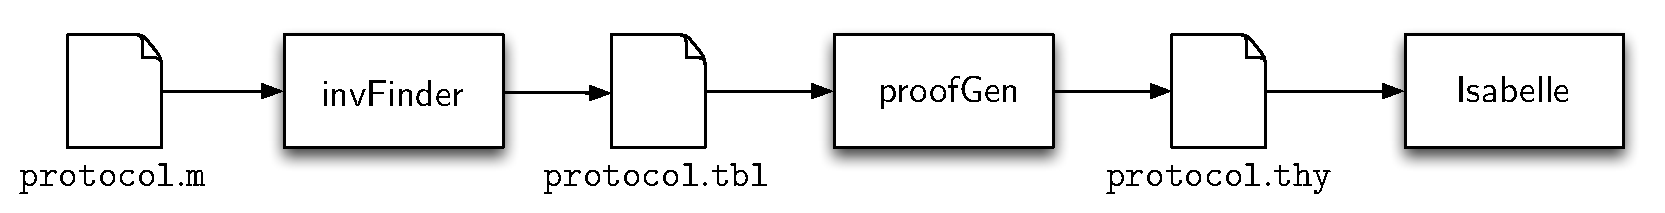
\includegraphics[width=1.0\textwidth]{paraVerifier.pdf}
%\vspace{-0.6cm}
%\caption{The workflow of {\sf paraVerifier}.}
%\label{fig:arch}
%\end{figure}
%\vspace{-0.8cm}

Our solutions to the two problems are as follows:
Given a protocol,  \texttt{invFinder} finds all the necessary ground auxiliary invariants from a small instance of the protocol in Murphi. This step solves the first  problem.
 A table {\tt protocol.tbl} is worked out  to store the set of ground invariants and
 causal relations, which are then  used by {\tt proofGen} to
create an Isabelle proof   script which models and verifies the
protocol in a parameterized form. In this step, ground invariants
are generalized into a parameterized form, and accordingly
ground causal relations are adopted to create parameterized
proof commands which essentially proves the existence of the
parameterized causal relations. This solves the second problem.  At last, the Isabelle proof script is
fed into Isabelle to check the correctness of the protocol.
%Consistency lemma has eliminated the need of directly use of usual induction proof method. Applying it, we  decompose the problem of invariant checking into that of checking the causal relation between $f$ and $r$ by case analysing parameters of a rule and an invariant. As shown in  and such a causal relation checking is within the ability of an automatical tactic provided by a theorem prover like Isabelle. Due to the uniform style of checking causal relation, it is also feasible to generate a proof of such a style by an external proof generator. However, as shown in Example \ref{example2}, the   three items shows that there are three subcases where we compare rule parameter $iR_1$ with formula parameters $i_1$ and $i_2$, different kinds of causal relations hold between rule $\mathsf{crit}~iR_1$ and invariant $\mathsf{mutualInv}~i_1~i_2$. Only if a proof script contains enough information on the case splitting and  which kind of causal relation to be checked in each case, Isabelle can help us to automatically  check whether the kind of causal relation hold in the case. How to provide these key proof information is a central problem in work of both {\sf invFinder} and {\sf proofGen}.
%\vspace{-0.6cm}

\section{  Searching Auxiliary Invariants}


\SetAlFnt{\small}

%\vspace{-0.8cm}

\begin{algorithm}\label{alg:invFinder}

\caption{Algorithm: $invFinder$}\label{alg:invfinder}

\KwIn{  Initially given invariants $F$, a protocol $\mathcal{P}=<I,R>$ }

\KwOut{A set of tuples which represent causal relations between concrete rules and invariants: }

{
    $A\leftarrow F$;

    $tuples \leftarrow []$;

    $newInvs \leftarrow F$;

    \While{$newInvs$ is not empty}
    {
   $ f \leftarrow newInvs.dequeue$;

   \For {$r \in R$}
   { $paras \leftarrow \mathsf{Policy}(r,f)$;

      \For {$para \in paras$}
     {$cr \leftarrow \mathsf{apply}(r,para)$;

       $newInvOpt,rel \leftarrow \mathsf{coreFinder}(cr,  f, A)$;

        $tuples \leftarrow tuples @[<r, para, f, rel>]$;

       \If{$newInvOpt \neq NONE$}
        {$newInv \leftarrow \mathsf{get}(newInvOpt)$\;
         newInvs.enqueue(newInv)\;
        $A \leftarrow A \cup \{newInv\}$\;
        }

     }
   }
  }
\Return $tuples$\;
}

%}

\end{algorithm}
%\vspace{-0.8cm}
Given a protocol $\mathcal{P}$ and a property set $F$ containing invariant formulas we want to verify, {\tt invFinder} aims to find useful auxiliary invariants and causal relations which are capable of proving any element in $F$.  A set $A$ is used to store all the invariants found up to now, and is initialized as  $F$. A queue  $newInvs$ is used to store new invariants which have not been checked,  and  is initialized as  $F$.  A relation table $tuples$ is used to record the causal relation between a parameterized rule in some parameter setting and a concrete invariant. Initially $tuples$ is set as NULL.
{\sf invFinder}  works iteratively in a semi-proving and semi-searching way. In each iteration, the head element $f$ of $newInvs$ is popped,  then $\mathsf{Policy}(r,f)$  generates groups of parameters $paras$  according to $r$ and $f$ by some policy. For each parameter $para$ in $paras$,   it is applied to instantiate $r$ into a concrete rule $cr$.  Here  $\mathsf{apply}(r,para)=r$ if $r$ contains no array-variables and $para=[]$; otherwise $\mathsf{apply}(r,para)=r(para_{[1]},..., para_{[|para|]})$. Then $coreFinder(cr,  f, A)$ is called to check
 whether  a causal relation exists between $cr$ and $f$; if there is such one relation item, the relation item $rel$ and a  formula option $newInvOpt$ is returned; otherwise a run-time error occurs in  $coreFinder$, which indicates no proof can be found. In the first case, a tuple $<r, para, f, rel>$ will be inserted into $tuples$; If the formula option $newInvOpt$ is $\mathsf{NONE}$, then no new invariant formula is generated; otherwise $newInvOpt=\mathsf{Some}(f')$ for some formula $f'$, then  $\mathsf{get}(newInvOpt)$ returns $f'$, and the new invariant formula $f'$ will be pushed into the queue $newInvs$ and inserted into the invariant set $A$.  The above searching process is executed until $newInvs$ becomes empty.  At last, the table $tuples$ is returned.

%instantiates the parameterized rule $r$ into a set of concrete rules $crs$ with different groups of concrete parameters Each rule in $crs$  represents a pattern w.r.t. the relationship (equivalent or not) between concrete rule parameters and invariant parameters. Such a parameter instantiation to the rule $pr$ can be generalized to a symbolic predicate {\bf which is according with a case (what do you mean?)}, as shown in Example \ref{example2}. Therefore, a good parameter instantiation policy should guarantee the completeness. Namely, each of subcases in the needed case-splitting should be covered by a concrete rule which is instantiated from $pr$ according to the policy.

%({\bf is this also accomplished by $coreFinder$? })\\
% \lyj{$CoreFinder$ only deal with a concrete rule $cr$ and a concrete invariant}

%For a rule $cr \in crs$ ({\bf for a rule and an invariant?}), {\sf invFinder} tries to prove that some causal relation exists between the rule and an invariant; if there is no such an invariant
%in the current invariant set, {\sf invFinder} automatically generates a new auxiliary invariant  and records the corresponding causal
%relation information between the current rule and invariant. %Note that the same causal relation should  hold between the generalized rule and invariant.
%Whenever a new invariant is generated, it is pushed into $newInvs$.  The above searching process is executed until $newInvs$ becomes empty. This searching process is a core algorithm of {\sf invFinder}, and we will describe it in Section 4.2, after introducing the parameter instantiation policy.


In Algorithm \ref{alg:invFinder}, the parameter generation policy $\mathsf{Policy}$  and the core invariant searching function $\mathsf{coreFinder}$ will be illustrated in Section \ref{sec:parameterGenPolicy} and \ref{sec:coresearchingAlgorithm}.

%\caicomment{The algorithm pseudo code is good. Try to make the description of invFinder consistent with pseudo code, and as simple as possible.}

\vspace{-0.5cm}
\subsection{Parameter Generation Policy}\label{sec:parameterGenPolicy}
In order to formulate our parameter generation policy, we introduce the concept of permutation modulo to symmetry relation $\simeq_m^n$,  and a quotient set of $\mathsf{perms}_{m}^{n}$ (the set of all $n$-permutations of $m$) under the  relation.  Here an $n$-permutation of $m$ is ordered arrangement of  an $n$--element subset of an $m$-element set $I=\{i. 0<i\le m\}$. We use a list $xs$ with size $n$ to stand for a $n$-permutation of $m$. For instance, $[1,2]$ is a 2-permutation of 3. $xs_{[i]}$ and $|xs|$  denote  the $i-$th element and the length of $xs$ respectively. If $xs_{[i]}=i$ for all $i \le |xs|$, we call it identical permutation. %, and sometimes is denoted by $1~ \mathsf{upto}~ n$ if $n=|xs|$.

\begin{definition}
Let $m$ and $n$ be two natural numbers, where $n \le m$,  $L$ and $L'$ are two lists which stand for two  $n$-permutations of $m$,
\begin{enumerate}[noitemsep,nolistsep]
\item
$L \sim_m^n L' \equiv (|L| =|L'|=n) \wedge (\forall i. i<|L| \wedge L_{[i]} \le m-n \longrightarrow L_{[i]}=L'_{[i]}) $.

\item $L \simeq_m^n L' \equiv L \sim_m^n L' \wedge   L' \sim_m^n L$.

%\item$[[L]]_{m}^{n} \equiv \{L'. L \in \mathsf{perms}_{m}^{n} \wedge L \sim_m^n L'\}$.

\item $\mathsf{semiP}(m,n,S)\equiv (\forall  L \in \mathsf{perms}_{m}^{n} \exists  L' \in S. L \simeq_m^n L' ) \wedge (\forall  L\in S. \forall L'\in S. L \neq L' \longrightarrow \neg  (L \simeq_m^n L' )$.

\item    A set $S$ is called a quotient of the set $\mathsf{perms}_{m}^{n}$ under the relation $\simeq_m^n$ if    $\mathsf{semiP}(m,n,S)$.
\end{enumerate}
\end{definition}

The definition of of relation $\simeq_m^n$ (item 1 and 2 in Definition 3) directly leads to the following lemma. %\caicomment{(Original version has a paragraph here to explain $L \simeq_{m+n}^n L' $. But the explanation is just a repetition of the below lemma while the lemma is more clear, from my viewpoint. So I delete them, and move the example downwards.)}

%According to the definition of of the relation $\simeq_m^n$, $L \simeq_{m+n}^n L' $ means that for any $0<i\le |L|$ and $0<j \le m$,
%if we compare any element $L_{[i]}$ with any $j\le m$, the comparison result is the same as that obtained by comparing $L'_{[i]}$ with $j$, namely
%$L_{[i]}=j$ if and only if $L'_{[i]}=j$ .
%For instance, let $L=[2,3]$ and $L'=[2,4]$, then $L \simeq_{4}^2 L' $. \cai{(should it be $\simeq_{6}^2$, since m+n=6 here)} This observation is formally captured by the following lemma. \cai{I simplify this paragraph, which focuses on the essential of $L \simeq_{m+n}^n L' $ }



\begin{lemma}\label{lemma:simeq1}%[(consistency lemma)]
If $L \simeq_{m+n}^n L' $, then for any $0<i\le |L|$, any $0<j \le m$, $L_{[i]}=j$ if and only if $L'_{[i]}=j$.
\end{lemma}

For instance, let $L=[2,3]$ and $L'=[2,4]$, then $L \simeq_{4}^2 L' $. %\caicomment{(should it be $\simeq_{6}^2$, since m+n=6 here)}
%\lyj{here is 4 ,not 6. Namely $m=4$,$n=2$. Thus $m-n=2$. Please recall Def 3, $L_{[1]}=2$, and $L_{[1]} \le 2$, thus $L_{[1]}'$ must be the same as $L_{[1]}$. But $L_{[2]}> 2$, we don not require $L_{[2]}' =L_{[2]}$.}
%\cai{Thanks to} Lemma \ref{lemma:simeq1},
Due to Lemma \ref{lemma:simeq1},
we can analyze a group of concrete parameters by analyzing only one of them as a presentative. Keeping this in mind, let us look at the following lemma, which together with Lemma \ref{lemma:simeq1} is the theoretical basis of our policy.


\begin{lemma}\label{lemma:simeqQuotinent}  Let $S $ be a set s.t.  $\mathsf{semiP}(m,n,S)$,
\begin{enumerate}[noitemsep,nolistsep]
\item \label{complete}  for any $L \in \mathsf{perms}_{m}^{n}$, there exists a $L' \in S$ s.t. $L \simeq_m^n L'$.
\item \label{distinct} let $L \in S$, $L' \in S$, if $L \ne L'$, then there exists two indice $i \le m$ and $j \le n$ such that $L_{[i]}=j$ and $L'_{[i]}\ne j$.
\end{enumerate}
\end{lemma}

Lemma \ref{lemma:simeqQuotinent} shows \ref{complete}) completeness of $S$ w.r.t. the set $\mathsf{perms}_{m}^{n}$ under the relation $\simeq$, \ref{distinct})  the distinction between two different elements in $S$. Therefore, $S$ has covered all analysing patterns according to the aforementioned comparing scheme between elements of $L$ with numbers $j<n-m$. Moreover, the case patterns represented by different elements in $S$ are different from each other. This fact can be illustrated by the following example.
\begin{example}
Let $m=2$, $n=1$, $S=\{[1],[2],[3]\}$ and  $\mathsf{semiP}(m,n,S)$,  let $LR$ be an element in $S$, there are three cases:
\begin{enumerate}[noitemsep,nolistsep]
%\begin{itemize}[noitemsep,nolistsep]
\item $LR=[1]$: it is a special case where $LR_{[1]}=1 $;
\item $LR=[2]$: it is a special case where $LR_{[1]}=2 $;
\item $LR=[3]$: it is a special case where $LR_{[1]}\ne 1$ and $LR_{[1]}\ne 2$.
%\end{itemize}
\end{enumerate}
\end{example}
Note that the above cases are mutually disjoint, and their disjunction  is true.

%Consider  natural numbers $m$ and $n$, computing a quotient of $\mathsf{perms}_{m}^{n}$ can be implemented by an algorithm $\mathsf{cmpSemiperm}$. Roughly speaking, $\mathsf{cmpSemiperm}$ firstly computes the set $\mathsf{perms}_m^n$, and push elements of it into a queue $S_0$, and select elements of $S_0$ into a set $S$. Initially $S$ is set empty. the head element of $S_0$ is pop into $L$, then $L$ will be checked whether there is an element $L'$ in $S$ s.t. $L\simeq_m^n L'$. If  yes, then $L$ will be discarded, else $L$ is inserted into $S$. This procedure is repeated until $S$ is empty. Finally $S$ will be returned. The detail of $\mathsf{cmpSemiperm}$ can be found in \cite{}.

%\caicomment{why introduce the following definition, need a guide for reader. E.g, we use normalized invariant as presentative of a group of invariants? }
%\lyj{this is a key problem, I revise my definition according to your comments}

In Algorithm \ref{alg:invFinder}, a concrete formula $cinv$ is poped from the queue $newInvs$, which can be seen as a normalized instantiation of some parameterized formula $pinv$. % A normalized instantiation can be seen as a representative of all instantiations of $pinv$.  For a parameterized rule $r$ and the  parameterized invariant $pinv$, we only probe  causal relations between some rule instances of $r$  and $cinv$.  Here a rule instance is obtained by instantiating $r$ with a parameter group $para$    in $paras$, which is generated according to the parameter generation policy.  A symbolic causal relation between $r$ and $pinv$ in a symbolic case can be generalized from a concrete causal relation existing between a concrete rule instance and the normalized invariant $cinv$.  Therefore $para$  can be used to derive a symbolic predicate such as  $i_1 \neq iR_1$, and $i_2 \neq iR_1$,  as shown in Example \ref{example2}.  Such a predicate  formulates a case  of comparing between rule parameters and invariant formula parameters. %A good parameter generation policy should guarantee the completeness. Namely, each of subcases in the needed case-splitting of the above parameters  comparing should be covered by the derivation of an element in the generated paramter groups $paras$.


\begin{definition}
A  concrete invariant formula $cinv$ is normalized w.r.t a parameterized invariant $pinv$ if  there exists no array variable in $cinv$ and $pinv=cinv$ or there exits an identical permutation $LI$ with $|LI|>0$ such that $cinv=pinv(1,...~|LI|)$;

\end{definition}

Any normalized $cinv$ containing array variables is obtained by instantiating a parameterized invariant $pinv$ with a parameter list which is an identical permutation $LI$ (i.e., the $j^{th}$ parameter is $j$ itself $LI_{[j]}=j$). Thus, consider a list of parameter $LR$ which is used to instantiate a parameterized rule $pr$, we  have $LR_{[i]}=j$ (or $LR_{[i]}\ne j$) is equivalent to $LR_{[i]}=LI_{[j]}$ (or $LR_{[i]}\ne LI_{[j]}$), %\lyj{my correction}{\bf[what is LR, you only use it in an example, need to define it clearly in this paragraph] },
which is a factor to specify a case by comparing $LR_{[i]}$ with $LI_{[j]}$ .  %All the auxiliary invariant formulas will be in a normalized form, and checked with any parameterized rule whether some kind of causal relation hold between them.


%{\bf Our Parameter Instantiation Policy:}
Let $cinv$  be a normalized concrete invariant w.r.t. a parameterized invariant $pinv$, $pr$ be a parameterized rule, $m$ be the number of actual parameters occurring in $cinv$, and $n$  be the number of formal parameters occurring in $pr$,  our policy is to compute a quotient of $\mathsf{perms}_{m}^{n}$, denoted as $\mathsf{cmpSemiperm}(m+n,n )$, and use elements of it as a group of parameters to instantiate $pr$ into a set $crs$ of concrete rules.\footnote{the details of computing $\mathsf{cmpSemiperm}(m+n,n )$ can be found in \cite{LiCache16}.}  For instance, for the invariant $\mathsf{mutualInv}(1,2)$, three groups of parameters [1], [2], [3] are used to instantiate $\mathsf{crit}$ respectively, each of the instantiation results will be used to check which kind of  causal relation exists between it and $\mathsf{mutualInv}(1,2)$.  Each of the three probed concrete causal relations will be used to generalized  into a symbolic causal relation existing between $\mathsf{crit}$ and $\mathsf{mutualInv}$ in a case formulated by a predicate comparing rule parameters and invariant parameters.  %A good parameter generation policy should guarantee the completeness. Namely, each of subcases in the needed case-splitting of the above parameters  comparing should be covered by the derivation of an element in the generated paramter groups $paras$.  In Section \ref{sec:generalization}, we will illustrate how three groups of parameters [1], [2], [3]  can be derived into three predicate which describes cases as shown in  Example \ref{example2}, which is a complete partition.

\subsection{Core Searching Algorithm}\label{sec:coresearchingAlgorithm}

\vspace{-0.3cm}
For a  $cinv$ and a rule $r \in crs$, the core part of the {\sf invFinder} tool is shown in Algorithm \ref{alg:invfinderI}. It needs to call two oracles. The first one, denoted by {\tt chk}, checks whether a ground formula is an invariant. Such an oracle can be implemented by translating the formula into a formula in SMV, and calling SMV to check whether it is an invariant  in a given small reference model of the protocol. If  the reference model is too small to check the invariant, then the formula will be checked by Murphi in a big reference model.  The second oracle, denoted by {\tt tautChk}, checks whether a formula is a tautology. Such a tautology checker is implemented by translating the formula into a form in the SMT (SAT Modulo Theories) format, and checking it by an SMT solver such as Z3.

%\vspace{-0.6cm}
\begin{algorithm}\label{alg:invFinder-I}

\caption{Core Searching Algorithm: $coreFinder$}\label{alg:invfinderI}

\KwIn{  $r$, $inv$, $invs$   }

\KwOut{A formula  option $f$, a new causal relation $rel$}

{
    $g\leftarrow $the guard of r, $S\leftarrow $the statement of r\;

    $inv'\leftarrow \mathsf{preCond}(inv, S)$\; \label{line:preCondComp}

    \If{$inv=inv'$}
    {
    $relItem\leftarrow (r, inv, invRule_2,-)$\;
    \Return $(\mathsf{NONE},  relItem )$\;
    }
    \ElseIf{$\mathsf{tautChk}(g\rightarrow inv')=true$}
    {
    $relItem\leftarrow (r, inv, invRule_1,-)$\;
    \Return $(NONE,  relItem )$\;
    }
    \Else
    {
    $candidates\leftarrow \mathsf{subsets}(\mathsf{decompose}(\mathsf{dualNeg}(inv')\andc g))$\;
    $newInv\leftarrow choose(chk,candidates)$\;
    $relItem\leftarrow (r, inv, invRule_3,newInv)$\;
    \If{$isNew(newInv,  invs)$}
    {
    $newInv \leftarrow  normalize(newInv)$\;%$ and insert it into the head of $newInvs$\;
    \Return $(\mathsf{SOME}(newInv),   relItem )$\;
    }
    \Else{\Return $(\mathsf{NONE},  relItem )$\;}
    }
}

%}

\end{algorithm}
%\vspace{-0.8cm}



%Besides the two oracles which are passed as parameters,
Input parameters of Algorithm \ref{alg:invFinder-I} include a rule instance $r$, an invariant $inv$, a sets of invariants $invs$.  The sets $invs$   stores the auxiliary invariants constructed up to now. The algorithm   searches for new invariants and    constructs the causal relation between the rule instance $r$ and the invariant $inv$.
The algorithm returns a formula option and a causal relation item between $r$ and $inv$. A formula option value $\mathsf{NONE}$ indicates that no new invariant is found, while $\mathsf{SOME}(f)$ indicates a new auxiliary invariant $f$ is searched.


%{\sf invFinder} is implemented by FL, which is an excellent STE-tool
%  The above function {\sf findInvsFromRule} tries to find new
%invariants and construct the causal relation between the rule
%instance $rule$. %The statement {\tt
%cond => te|fe} is an abbreviation of the if-then-else expression
%that if $cond$ is true then $te$ else $fe$.
%Parameters $newInvs$, $invs$, and $casRel$ are new invariants, invariants, and all the
%causal relations constructed up to now, the above oracle functions
%are also passed as parameters.  % Causal relations  are still not
%checked between the ones in $newInvs$ and rules.
%

Algorithm $coreFinder$ works as follows: after computing the pre-condition $ inv'$ (line \ref{line:preCondComp}), which is the weakest precondition of the input formula $inv$ w.r.t. $S$, the algorithm takes further operations according to the cases it faces with:
%Algorithm {\sf invFinder-I} performs case analysis on $inv'$:

\begin{description}
\item[(1)] If $ inv=inv'$, meaning that statement $S$ does not change $inv$, then no new invariant is created, and  new causal
relation item marked with tag {\tt invHoldRule$_2$} is recorded
between $r$ and $inv$.% but at this moment there are no new invariants to be added; %for instance, let $ r=\mathsf{crit} (3)$,  $ inv=\mathsf{mutualInv}(1,2)$, thus
%$inv'=\mathsf{preCond}(S,inv)=inv$, then a pair  $ (\mathsf{NONE}, ( crit(3), inv, \mathsf{invHoldRule}_2,\_))$ will be returned, where $NONE$ means no new invariant formula is returned.

\item[(2)] If $\mathsf{ tautChk}$ verifies that $g \dashrightarrow inv'$ is a tautology, then  no new invariant is created, and
the new causal relation item marked with tag
$ \mathsf{invHoldRule}_1$ is recorded between $r$ and $inv$. %For instance, let $r=\mathsf{crit}(2)$, $inv=\mathsf{invOnXC}(1)$,
% $inv'=\mathsf{preCond}(S,inv)=\neg(\mathsf{false }\eqc \mathsf{true} \andc n[1] \eqc \mathsf{C})$, obviously, $
%g \dashrightarrow inv'$ holds forever because $inv'$ is always evaluated true,
% thus a pair $(\mathsf{NONE},  (\mathsf{crit}(2), inv, \mathsf{invHoldRule}_1,\_))$ will be returned.


\item[(3)] If neither of the above two cases holds, then a new auxiliary invariant $newInv$ will be constructed, which will make the causal relation $ \mathsf{invHoldRule}_3$  to hold. The candidate set is $subsets(decompose(dualNeg(inv')\andc g))$, where $decompose(f)$ decompose $f$ into a set of sub-formulas $f_i$  such that each $f_i$ is not of a conjunction form and $f$   is semantically equivalent to $f_1 \andc f_2 \andc ... \andc f_N$. $dualNeg(\negc f)$ returns $f$. $subsets(S)$ denotes the power set of $S$.
%The construction of the auxiliary invariant is introduced better after giving some definitions. A formula $f$ can be composed into a set of sub-formulas $f_i$, denoted as $decompose(f)$, such that each $f_i$ is not of a conjunction form and $f$   is semantically equivalent to $f_1 \andc f_2 \andc ... \andc f_N$.  $f_i$ usually is an atomic formula in our work after decomposition. For a formula $f$, we use $subsets(f)$ to denote the power set of $decompose(f)$, which contains all subsets of $decompose(f)$. $dualNeg(\negc f)$ returns $f$. The $\mathsf{ normalize}(f)$ function normalizes the numbering order of the use of parameters in the invariant $inv$.
%The result formula should be in  a normal form, whose parameters
%  always start from 1, and increase one by one if there are more
%  parameters. E.g.,  $\negc (x\eqc\mathsf{true} \andc n[1]\eqc\mathsf{C})$ is normalized, but
%  $\negc (x\eqc\mathsf{true} \andc n[2]\eqc\mathsf{C})$  not. The implementation of $\mathsf{ normalize}$ firstly compute a protype of $f'$,  which is obtained by substituting concrete parameters with different  e index variables $i_1$, ...$i_n$ in a pre-order traversal of the syntax of $f$, where $n$ is  the number of concrete parameters occurring in $f$ , then the returned result by $normalize$ is the formula which is obtained by substituting index variables $i_1$, ...$i_n$ with concrete indexes 1,...,$n$. Namely, we can see a normalized formula is obtained by substituting formal index variables with an identical permutation $1~ \mathsf{upto}~ n$.
A proper formula is chosen from the candidate set to construct a new invariant $newInv$. This is accomplished by the {\tt choose} function, which calls the oracle {\tt chk} to verify whether a formula is an invariant in the given reference model. After $newInv$ is chosen, the function $isNew$ checks whether this invariant is new w.r.t. $newInvs$ or $invs$. If this is the case, the invariant will be normalized, and then be  added into $newInvs$, and the new causal relation item marked with tag {\tt invRule$_3$} will be added into the causal relations. The meaning of the word ``new" is modulo to the symmetry relation. E.g., $\mathsf{mutualInv}(1,2)$ is equivalent to
$\mathsf{mutualInv}(2,1)$ in a symmetry view. % Let $ invs=\emptyset$, $ r=\mathsf{crit}(1)$, $ inv=\mathsf{mutualInv}(1,2)$,
%$ inv'= \mathsf{preCond}(S,inv)=\negc(true\eqc true \andc n[2]\eqc C)$, from all the subsets of $\{n[1]\eqc T, x\eqc true, n[2]\eqc C\}$, the $ \mathsf{choose}$ oracle selects the subset $\{ x=true, n[2]\eqc C\}$ combines all the item in this candidate, then constructs a new invariant $inv_0= \negc(x\eqc true \andc
 %  n[2]\eqc C)$. After   normalization, the new invariant   $\negc(x=true \andc
%   n[1]\eqc C)$  and  a  relation item $ (crit(1),   \mathsf{invHoldRule}_3, inv_0)$ will be returned.


\end{description}

%Roughly speaking, the top level of {\sf invFinder} works as follows: a queue  $newInvs'$ is used to store new invariants found, and the initial value of $newInvs'$ is set by the initial invariant formulas we want to verify. Head element of $newInvs'$ is pushed, and used to check the consistency relation with all the parameterized rules.  $\mathsf{InvFinder}$ is iteratively called to compute new invariant formulas and relation items. This searching procedure is not finished until no new invariant is searched.

\vspace{-0.5cm}
 \begin{table}[htbp]
\centering \caption{A fragment of output of {\sf invFinder}\label{table:groundCausalRelation}} % {\tt
%simpMutual.tbl}
\begin{tabular}{|c|c|c|c|c|  }
\hline
  rule& ruleParas&inv&causal relation &   f'  \\
\hline
  .. & ..&.. &..&.. \\

\hline
  crit  & [1]&mutualInv(1,2)& invHoldRule3 &invOnXC(2) \\
\hline
  crit &[2]& mutualInv(1,2)& invHoldRule3 &invOnXC(1)  \\
\hline
  crit & [3]& mutualInv(1,2) & invHoldRule2  & \\
\hline
  .. & ..&.. &..&.. \\

\hline
  crit  & [1]&invOnXC(1) & invHoldRule1 &\_ \\
\hline
  crit &[2]& invOnXC(1) & invHoldRule1 &\_  \\
\hline
\end{tabular}
\end{table}

%\vspace{-0.8cm}

For instance, let $PR=\{try, crit, exit, idle\}$, $invs=\{mutualInv(1,2)\}$,    the output of the {\sf invFinder}, which is stored in file {\tt mutual.tbl},  is shown in Table
\ref{table:groundCausalRelation}. In the table,  each line records the    index of a normalized   invariant, name of a parameterized rule, the rule
  parameters to instantiate the rule, a causal relation between
  the ground invariant and a kind of causal relation which involves the kind and proper formulas
  $f'$   in need (which are used to construct
      causal relations $\mathsf{invHoldRule}_3$). The auxiliary invariants found by {\sf invFinder} include: $\mathsf{inv_2}  \equiv  \negc (\mathsf{x} \eqc \mathsf{true}  \andc  n[1]=\mathsf{C})$, $\mathsf{inv_3}    \equiv \negc  ( n[1]=\mathsf{C} \andc n[2]=\mathsf{E})$,
$\mathsf{inv_4}  \equiv  \negc (x \eqc \mathsf{true}  \andc  n[1]\eqc \mathsf{E})$,   $\mathsf{inv_5}    \equiv \negc  ( n[1]\eqc \mathsf{E} \andc n[2] \eqc \mathsf{E})$.  \footnote{The names $\mathsf{mutualEx}$ and $\mathsf{invOnX1}$ in
  this work are just for easy-reading, their
 index here is generated  in some order by {\sf invFinder}}.


%\vspace{-0.5cm}
\section{Generalization}\label{sec:generalization}
%\vspace{-0.5cm}%From this section, our modelling language has been extended to HOL (Higher-order Logic) provided by Isabelle, which not only include the language in Section \ref{sec:protocolSyntax}, but also higher-order logic features. This is not surprising because our formal theory for a parameterized instance of a protocol is done in HOL/Isabelle.  In order to include the theory formally in section \ref{sec:protocolSyntax} and \ref{sec:causal_rel}, we define a Isabelle theory {\tt cache.thy}.
Intuitively, generalization means that a concrete index (formula or rule) is generalized into a set of concrete indices (formulas or rules), which can be formalized  by a symbolic index (formula or rules) with side conditions  specified by   constraint formulas.     In order to do this, we  adopt a new constructor  to model symbolic index or symbolic value $\mathsf{symb}(str)$, where $str$ is   a string.  We use $\mathtt{N}$ to denote $symb("N")$, which formalizes the size of an parameterized protocol instance. A concrete index $i$ can be transformed into a symbolic one by some special strategy $g$, namely  $\mathsf{symbolize}(g,i)=\mathsf{symb}(g(i))$. In this work, two special transforming function $\mathsf{fInv}(i)="iInv"\cat \mathsf{itoa}(i)$ and $\mathsf{fIr}(i)="iR"\cat \mathsf{itoa}(i)$, where $\mathsf{itoa}(i)$ is the standard function transforming an integer $i$ into a string. We use  special symbols $\mathtt{\iInv_i}$  to denote $\mathsf{symbolize}(fInv,i)$;  and $\mathtt{\iR_i}$ to denote $\mathsf{symbolize}(fIr,i)$. The former formalizes a symbolic parameter of a parameterized   formula, and the latter    a symbolic  parameter of a parameterized rule. Accordingly, we define $\mathsf{symbolize2f}(g,inv)$ (or  $\mathsf{symbolize2r}(g,r)$), which returns the symbolic transformation result to a concrete formula $inv$ (or rule $r$) by replacing a concrete index $i$ occurring in $inv$ (or $r$) with a symbolic index $\mathsf{symbolize}(g,i)$.


There are two
main kinds of generalization in our work: (1) generalization of a normalized invariant into a symbolic one. %This generation will be used for the generation of \cai{(replace to:
The resulting symbolic invariants are used to create definitions of invariant formulas in Isabelle. For instance,  $\negc$(x $\doteq$ true $\andc$ n[1]$\doteq$ C) is generalized into $\negc$(x $\doteq$ true $\andc$ n[$\mathtt{\iInv_1}$]$\doteq$ C).  This kind of generalization is done with model constraints, which  specify  that any parameter index should be not greater than the instance size $\mathtt{N}$, and parameters to instantiate a parameterized rule (formula) should be different. (2) The generalization of concrete causal relations into parameterized causal relations in Isabelle, and will be used in proofs of the existence  of causal relations in Isabelle.


Since the first kind of generalization is simple, we focus on the second kind of generalization, which consists of two phases.
Firstly, groups of rule parameters  such as [[1],[2],[3]] will be generalized into a list of  symbolic formulas  such as $[\mathtt{\iR_1} \eqc \mathtt{\iInv_1},\mathtt{\iR_1} \eqc \mathtt{\iInv_2},  (\mathtt{\iR_1} \ne \mathtt{\iInv_1}) \wedge  (\mathtt{\iR_1} \ne \mathtt{\iInv_2})] $\footnote{$\mathtt{\iR_1} \ne \mathtt{\iInv_1}$ is the abbreviation of $!(\mathtt{\iR_1} \eqc \mathtt{\iInv_1})$} , which  stands for case-splittings  by comparing  a symbolic rule parameter $iR_1$ and invariant parameters $\iInv_1$ and $\iInv_2$. In the second phase, the formula field accompanied with a $\mathsf{invHoldRule3}$ relation is also  generalized by some special strategy.  %This generation is prepared for the generation of proofs of the existence of causal relations in Isabelle. Here we focus on  %These formulas should be formalized in HOL.

Now let us look at the first phase, starting with some definitions.
Consider a line of concrete causal relation shown in Table \ref{table:groundCausalRelation}, there is a group of rule parameters $LR$, and a group of parameters $LI$ occurring in an  invariant formula.

\begin{definition}
Let $LR$ be a permutation s.t. $|LR|>0$, which represents a list of actual parameters to instantiate a parameterized rule,    let $LI$  be a  permutation $|LI|>0$,  which  represents a list of actual parameters to instantiate a parameterized invariant, we define:
\begin{enumerate}[noitemsep,nolistsep]
\item symbolic comparison condition generalized from comparing $LR_{[i]}$ and $LI_{[j]}$: \\
$ \mathsf{symbCmp}(LR,LI,i,j)\equiv $
 \begin{numcases}{ }
 \mathtt{\iR_i} \eqc \mathtt{\iInv_j} &   if $LR_{[i]}=LI_{[j]}$\ \ \ \ \\
\mathtt{\iR_i} \ne \mathtt{\iInv_j} & otherwise
\end{numcases}
%$symbCmp(LR,LI,i,j)\equiv$ if $equality(LR,LI,i,j)$ then $\mathtt{\iR_i} = \mathtt{\iInv_j}$ else $ (\mathtt{\iR_i} \ne \mathtt{\iInv_j})$

\item symbolic comparison  condition generalized from comparing   $LR_{[i]}$ and with all $LI_{[j]}$ :\\
$\mathsf{symbCaseI}(LR,LI,i)\equiv $\\
\begin{numcases}{ }
   symbCmp(LR,LI,i,j)& if $\exists! j.  LR_{[i]}=LI_{[j]}$\\
   forallForm(|LI|,pf)& otherwise
 \end{numcases}
 where  $pf(j)= \mathsf{symbCmp}(LR,LI,i,j)$, and $\exists!j.P$ is an qualifier meaning that  there exists a unique $j$ s.t. property $P$;

\item symbolic case  generalized from comparing $LR$ with $LI$ : $\mathsf{symbCase}(LR,LI )\equiv \mathsf{forallForm}(|LR|,pf)$, where $pf(i)= \mathsf{symbCaseI}(LR,LI,i )$;

\item symbolic partition generalized from comparing all $LRS_{[k]}$ with $LI$, where $LRS$ is a list of permutations with the same length: $\mathsf{partition}(LRS,LI) \equiv \mathsf{existsForm}(|LRS|,pf)$,  where $pf(i)= \mathsf{symbCase}(LRS_i,LI)$.

\end{enumerate}
\end{definition}

$\mathsf{symbCmp}(LR,LI,i,j)$ defines a symbolic formula  generalized from comparing $LR_{[i]}$ and $LI_{[j]}$; $\mathsf{symbCaseI}(LR,LI,i)$  a symbolic formula summarizing the results of comparison  between $LR_{[i]}$  and all $LI_{[j]}$ such that $j \le |LI|$; $\mathsf{symbCase}(LR,LI )$ a symbolic formula representing a subcase generalized from comparing all $LR_{[i]}$  and all $LI_{[j]}$; $\mathsf{partition}(LRS,LI)$  is a disjunction of subcases $\mathsf{symbCase}(LRS_{[i]},LI )$.  Recall the first three lines in Table. \ref{table:groundCausalRelation}, and $LI=[1,2]$ is the list of parameters occurring in $\mathsf{mutualEx}(1,2)$; and $LR$ is the actual parameter list to instantiate $\mathsf{crit}$.
 %\begin{itemize}
 %\item when   $LI=[1]$ is a list of parameters occurring in $invOnXC(1)$
%\begin{itemize}
 % \item $LR=[1]$ is the actual parameter list to instantiate $crit$, $symbCmp(LR,LI,1,1)=(\mathtt{\iR_1} = \mathtt{\iInv_1})$, $symbCase(LR,LI)=symbCaseI(LR,LI,1)=(\mathtt{\iR_1} = \mathtt{\iInv_1})$.

 % \item  $LR=[2]$ is the actual parameter list to instantiate $crit$, $symbCmp(LR,LI,1,1)= (\mathtt{\iR_1} \ne \mathtt{\iInv_1})$, $symbCase(LR,LI)=symbCase(LR,LI,1)=(\mathtt{\iR_1} \ne \mathtt{\iInv_1})$

  % \item let $LRS=[[1],[2]]$, $partition(LRS,LI)= (\mathtt{\iR_1} = \mathtt{\iInv_1}) \vee  (\mathtt{\iR_1} \ne \mathtt{\iInv_1})$
%\end{itemize}
%\item when   $LI=[1,2]$ is a list of parameters occurring in $mutualEx(1,2)$
\begin{itemize}[noitemsep,nolistsep]

  \item when $LR=[1]$, $\mathsf{symbCmp}(LR,LI,1,1)=(\mathtt{\iR_1} \eqc \mathtt{\iInv_1})$, $\mathsf{symbCase}(LR,LI)=\mathsf{symbCaseI}(LR,LI,1)=(\mathtt{\iR_1} \eqc \mathtt{\iInv_1})$ becuase $LR_{[1]}=LI_{[1]}$.

  \item when $LR=[2]$, $\mathsf{symbCmp}(LR,LI,1,2)= (\mathtt{\iR_1} \eqc \mathtt{\iInv_2})$, $\mathsf{symbCase}(LR,LI)=\mathsf{symbCaseI}(LR,LI,2)=(\mathtt{\iR_1} \eqc \mathtt{\iInv_2})$ becasue $LR_{[1]}=LI_{[2]}$.


 \item when  $LR=[3]$, $\mathsf{symbCmp}(LR,LI,1,1)=(\mathtt{\iR_1} \ne \mathtt{\iInv_1})$, $\mathsf{symbCmp}(LR,LI,1,2) = (\mathtt{\iR_1} \ne \mathtt{\iInv_2})$, $\mathsf{symbCase}(LR,LI)=symbCaseI(LR,LI,1)= (\mathtt{\iR_1} \ne \mathtt{\iInv_1}) \wedge  (\mathtt{\iR_1} \ne \mathtt{\iInv_2})$ because neither $LR_{[1]}=LI_{[1]}$ nor $LR_{[1]}=LI_{[2]}$.

  \item let $LRS=[[1],[2],[3]]$, $\mathsf{partition}(LRS,LI)= (\mathtt{\iR_1} \eqc \mathtt{\iInv_1}) \vee (\mathtt{\iR_1} \eqc \mathtt{\iInv_2}) \vee ( (\mathtt{\iR_1} \ne \mathtt{\iInv_1}) \wedge  (\mathtt{\iR_1} \ne \mathtt{\iInv_2}))$
\end{itemize}
%\end{itemize}

%Note that $\mathsf{partition}(LRS,LI)$ is a complete partition if it is a tautology.
%In the above example, the two partitions are both complete.
If we see a line  in table \ref{table:groundCausalRelation} as a concrete test case for some concrete causal relation,  then $\mathsf{symbCase}(LR, LI)$ is an abstraction predicate to generalize the concrete case. Namely, if we transform $\mathsf{symbCase}(LR, LI)$ by substituting $\mathtt{\iInv_i}$ with $LI_{[i]}$, and $\mathtt{\iR_j}$ with $LR_{[j]}$, the result is semantically equivalent to true. %If another $LR'$ and $LI'$ are permutations s.t.  $symbCase(LR', LI')$, then the same kind of causal relation  should hold, thus we can apply the same proof tactics to prove.

The second phase of generalization of concrete causal relations is to generalize the formula $inv'$ accompanied with a causal relation $\mathsf{invHoldRule_3}$ in a line of table \ref{table:groundCausalRelation}. An index occurring in $f'$ can either  occur in the invariant formula, or in the rule. We need to look it up to determine the  transformation.

\begin{definition}
Let $LI$ and $LR$ are two permutations,  $\mathsf{find\_first}(L,i)$ returns the least index $j$ s.t. $L_{[i]}=j$ if there exists such an index; otherwise returns an error.
%$\mathsf{lookup}(LI,LR, i)\equiv$
\begin{numcases}{\mathsf{lookup}(LI,LR, i)\equiv }
 \mathtt{\iInv_{find\_first(LI,i)}} &   if $i\in LI$\\
\mathtt{iR_{find\_first(LR,i) }} & otherwise
\end{numcases}
 %if $i\in LI$ then $\mathtt{\iInv_{find\_first(LI,i)}}$ else $\mathtt{iR_{find\_first(LR,i) }}$
%$\mathsf{symbolize'}(f,LI,LR) $ is a formula transformed from $f$ by substituting each $i$ with $lookup(LI,LR, i)$.
\end{definition}

$\mathsf{lookup}(LI,LR, i)$ returns the symbolic index transformed from $i$ according to whether $i$ occurs in $LI$ or in $LR$. The index $i$ will be transformed into  $\mathtt{\iInv_{find\_first(LI,i)}}$ if $i$ occurs in $LI$, and  $\mathtt{iR_{find\_first(LR,i) }}$ otherwise. Employing the $\mathsf{lookup}$ strategy to transform a concrete index $i$ in  $inv'$ to $\mathsf{lookup}(LI,LR, i)$, $\mathsf{symbolize2f}$ transforms $inv'$ into a symbolic one  which will be needed in a proof command for existence of the $\mathsf{invHoldRule_3}$  relation in Isabelle.  %\caicomment{not clear: $\mathsf{symbolize2f}$ calling $\mathsf{lookup}$ strategy   will be used  to transform   $inv'$ into  a symbolic formula, which will be needed for the generation of a proof command for existence of the $\mathsf{invHoldRule_3}$  relation in Isabelle.}
%For instance, let $LI=[1,2]$, $LR=[2]$, then  $\mathsf{lookup}(LI,LR, 2)=\mathtt{\iInv_2}$, and  $\mathsf{invOnXC}(2)$ is transformed into $\negc(x\eqc true \wedge n[\mathtt{\iInv_2}]\eqc C)$ by the strategy $\mathsf{lookup}$.

%Let $LI=[1]$, $LR=[1,2]$, then $symbolize'(mutualInv(1,2),LI,LR)$ is $\neg(n[\iInv_1]\eqc C \wedge n[\iR_2]\eqc C)$. Here the latter exmple is only  artificial because there is no rule which will be instantiated by $[1,2]$. But for complex protocols like FLASH, the case exits where a rule with two parameters and an invariant with only a parameter exits.
%For convenience in generating Isabelle proofs,      %a formula $\mathsf{diffConGen}~(\mathsf{paraMumsOfInv}~cr~"iR"$ to specify with the assumptions that mutual difference between the parameters of the symbolic invariant.  Here we assume that the string $"iR"$ does not occur in $cr$.
%a table $symbCausalTab$ is generated, which  stores causal relation between a parameterized rule and an  invariant w.r.t. a  size $N$. An entry of the table is referenced by concatation of the name of a rule and an invariant formula. Such an entry is a record containing fields {\tt symbCases} and  {\tt relationItems}, and created by collecting all the lines on the concrete relation items between the rule and the invariant. {\tt symbCases}  stores the list of symbolic cases each of which is derived by $\mathtt{symbCase}(LR, 1~\mathsf{upto}~n)$, where $LR$ is the rule parameters, and $n$ the number of parameters occurring in the invariant. relations store a list of generalized causal relation items.  For instance, for the rule $\mathsf{crit}$ and $\mathsf{inv5}$, a record $(|\mathtt{symbCases}=[\mathtt{\iR_1} = \mathtt{\iInv_1},\mathtt{\iR_1} = \mathtt{\iInv_2},(\mathtt{\iR_1} \ne \mathtt{\iInv_1}) \wedge  (\mathtt{\iR_1} \ne \mathtt{\iInv_2})]$; $\mathtt{relationItems}= [\mathsf{invHoldRule}_3(f_1')$,$\mathsf{invHoldRule_3}(f_2')$,$\mathsf{invHoldRule}_2]|)$, where $f_1'=\negc(x\eqc true \wedge n[\mathtt{\iInv_2}]\eqc C)$, and $f_2'=\negc(x\eqc true \wedge n[\mathtt{\iInv_1}]\eqc C)$.

%\vspace{-0.3cm}
%-------------------------------------------------------------------------
\section{Automatical Generation of Isabelle Proof }
%-------------------------------------------------------------------------
%\subsection{An  Example of Generated Isabelle/Script} \label{subsection:introOfIsabelleProof}
%\vspace{-0.3cm}
A formal model for a protocol case in a theorem prover like Isabelle
includes the definitions of constants and rules and invariants,
lemmas, and proofs. Readers can refer to \cite{LiCache16} for detailed illustration of the formal proof script. In this section, we focus on the generation of a lemma on the existence of causal relation between a parameterize rule and invariant formula based on the aforementioned generalization of lines of concrete causal relations. %An overview of the hierarchy  of the formal proof scripts of  is
%shown in Fig \ref{fig:isabelleProofIntro}.

%\begin{figure}[htbp]
% \centering %
% \vspace{-0.8cm}
%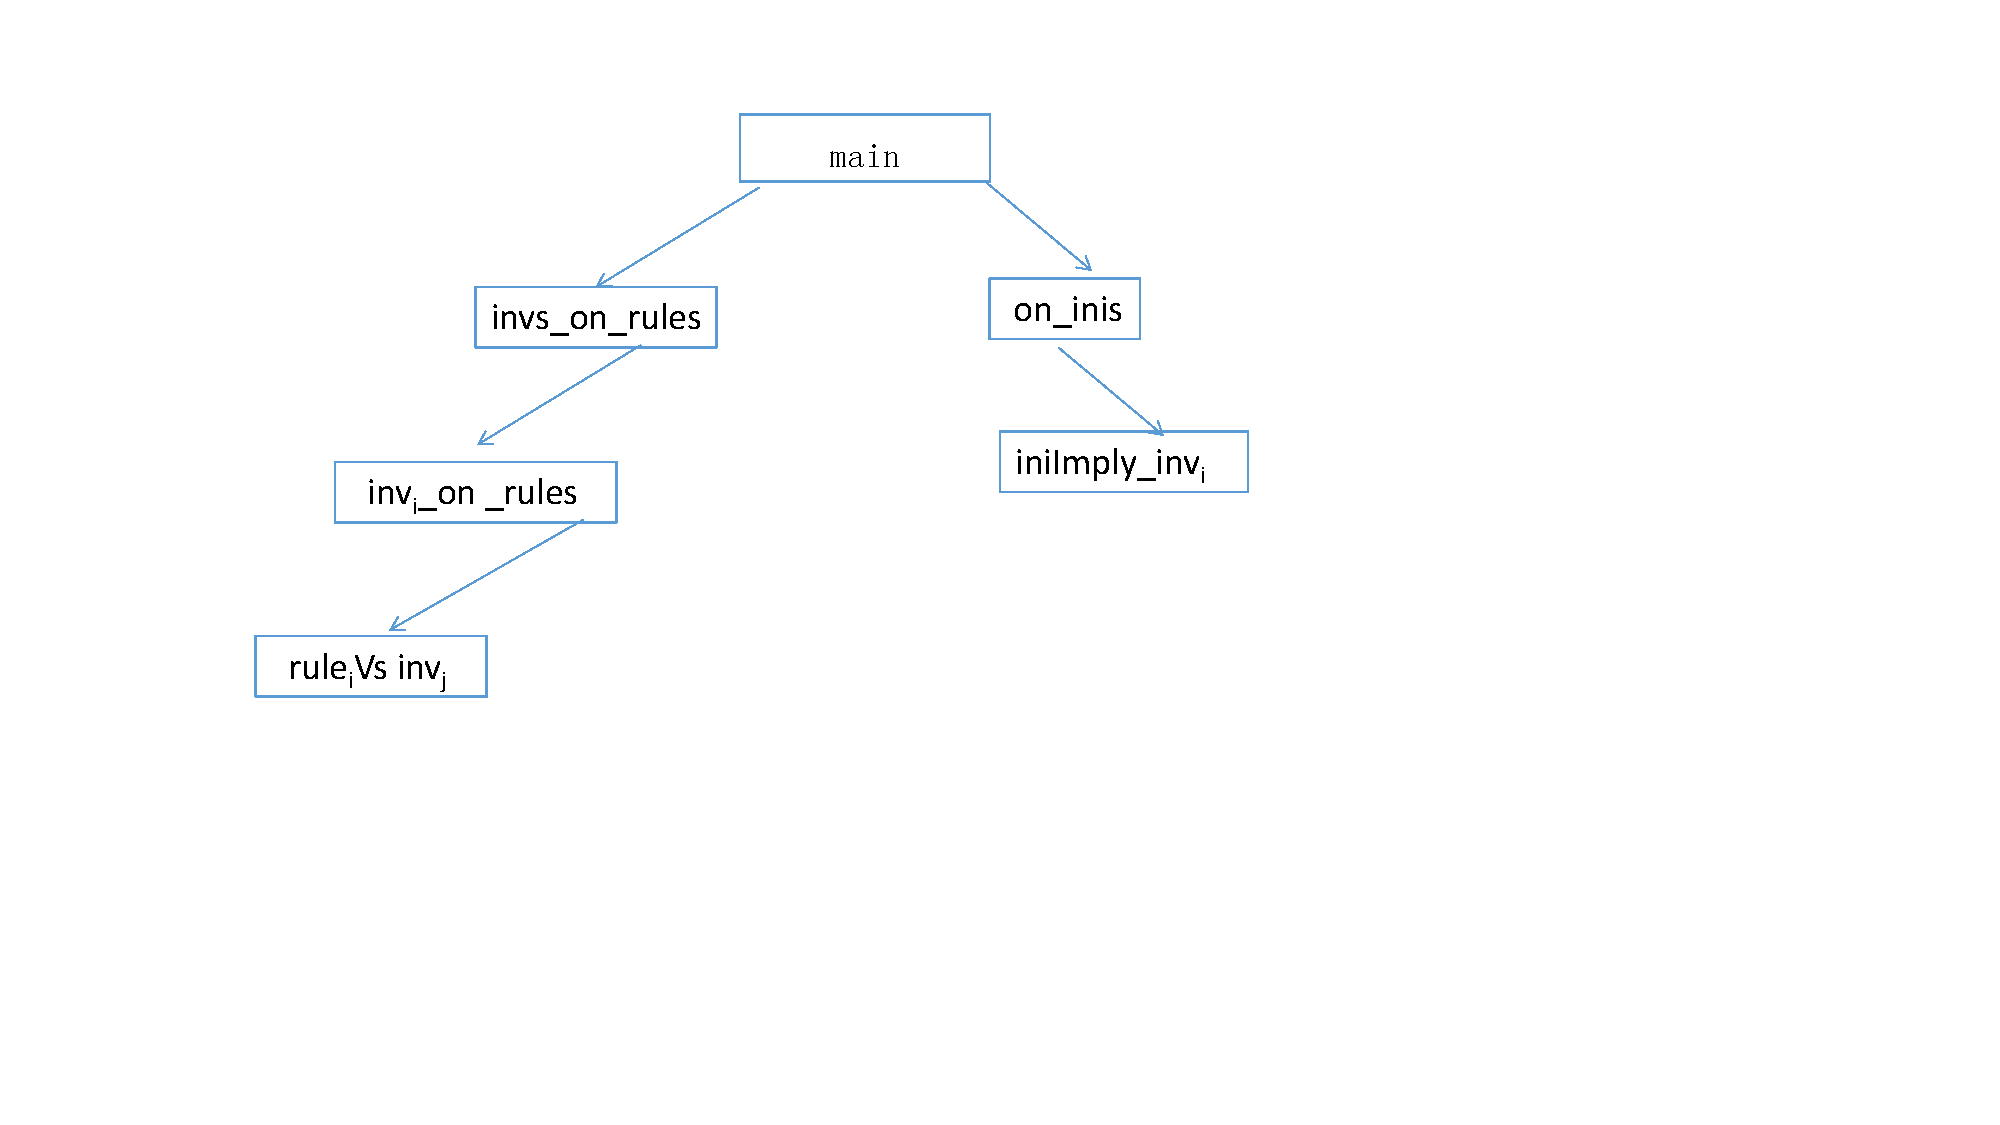
\includegraphics[width=1.0\textwidth]{lemmaHierachy}
%\vspace{-0.5cm}
%\caption{An overview of an Isabelle proof\label{fig:isabelleProofIntro}}

%\end{figure}

%In detail, the proof script is divided into   parts as follows: (1) Definitions of protocol under case study including enumerating datatypes; definitions of formally parameterized invariant formulas, and the set of all actual invariants w.r.t. a protocol instance; definitions of formally parameterized rules, and the set of all actual rules w.r.t. a protocol instance; definitions of specification of the initial state; (2) A lemma  such as {\tt rule$_i$Vsinv$_j$} on a causal relation of a rule and an invariant; (3) A  Lemma  such as {\tt inv$_i$OnRules} on causal relations for all rules in  the rule set  and an invariant. (4) A lemma {\tt invsOnRules} on a causal relation for all rules in  the rule set  and all invariants in the invariant set. (4) A Lemma such as {\tt iniImply\_inv$_i$} on a fact that an invariant {\tt inv$_i$}  holds at the initial state defined by the specification of the initial state. (5) A lemma {\tt on\_inits} proves that for all invariants they hold at the initial state of the protocol. (6) Main theorem  proving that any invariant formula  holds at any reachable state of the  N-parameterized the protocol instance.
%\subsubsection{Lemmas for Causal Relation between Rules and Invariants}
 % Now we discuss how to use records on {\tt crit} and {\tt inv$_1$} in the tables   $symbInvs$, $symbRules$, and $symbCausalTab$ to generate a lemma to prove that causal relation hold between   crit and   $inv_1$, which will be applied in the proof of main lemma.
 %A lemma at the bottom level, specifies that causal relation hold between  a rule like  $\mathsf{crit}$ and a parameterized rule like  $\mathsf{inv_1}$,
 An  example lemma
{\tt critVsinv$_1$} and its proof in Isabelle in the {\tt mutualEx} protocol, is illustrated as follows:

\begin{specification}
%\begin{algorithm}
%\caption{Generating a kind of proof which is according with a relation tag of $invHoldRule_{1-3}$ : rel2proof}\label{lemma:causal relation lemma}
1lemma critVsinv1:\\
2  assumes  a1: $\exists$ \iR1. \iR1 $\le$ N $\wedge$ r=crit \iR1 and \\
  a2: $\exists$  \iInv1 \iInv2. \iInv1 $\le$ N $\wedge$ \iInv2 $\le$ N $\wedge$ \iInv1 $\neq$ \iInv2 \\
   $\wedge$ f=inv1  \iInv1 \iInv2\\
3  shows  invHoldRule s f r (invariants
  N)\\
4  proof -\\
   from a1 obtain \iR1 where a1:\iR1 $\le$ N $\wedge$ r=crit \iR1 \\
\twoSpaces   by blast\\
   from a2 obtain \iInv1 \iInv2 where \\
   a2: \iInv1 $\le$ N $\wedge$ \iInv2 $\le$ N $\wedge$ \iInv1 $\neq$ \iInv2 $\wedge$ f=inv1  \iInv1 \iInv2\\
\twoSpaces   by blast \\
5  have iR1=\iInv1 $\vee$ \iR1=\iInv2 $\vee$ (\iR1 $\ne$ \iInv1 $\wedge$  \iR1 $\ne$ \iInv2) \\
  by auto\\

6  moreover\{assume  b1:\iR1=\iInv1\\
7  \twoSpaces have invHoldRule3 s f r (invariants N)\\
 \twoSpaces  \twoSpaces   proof(cut\_tac a1 a2 b1, simp, \\
 rule\_tac x=$\negc$ (x=true $\andc$ n[\iInv2]=C)  in exI,auto)qed\\
8  \twoSpaces then have invHoldRule s f r
(invariants
  N)
by auto\}\\

9  moreover\{assume  b1:iR1=\iInv2\\
10 \twoSpaces have invHoldRule3 s f r (invariants N)\\
 \twoSpaces \twoSpaces   proof(cut\_tac a1 a2 b1, simp, \\
 rule\_tac x=$\negc$ (x=true $\andc$ n[\iInv1]=C  in exI,auto)qed\\
11 \twoSpaces then have invHoldRule s f r (invariants
  N)
by auto\}\\

12   moreover\{assume  b1:(\iR1 $\ne$  \iInv1 $\wedge$   \iR1 $\ne$  \iInv2)\\
13 \twoSpaces have invHoldRule2 s f r  \\
  \twoSpaces \twoSpaces  proof(cut\_tac a1 a2 b1,  auto) qed\\
14 \twoSpaces then have invHoldRule s f r
(invariants
  N)
by auto\} \\

15ultimately show invHoldRule s f r
(invariants N) by blast\\
16qed\\
%\end{algorithm}
\end{specification}

In the above proof, line 2 are assumptions on the parameters of the invariant and rule, which are composed of two parts: (1) assumption {\tt a1} specifies that there exists an actual parameter {\tt \iR1} with which {\tt r} is a rule obtained by instantiating {\tt crit}; (2) assumption {\tt a2} specifies that  there exists   actual parameters {\tt \iInv1} and {\tt \iInv2} with which {\tt f} is a formula obtained by instantiating {\tt inv1}.
 %(1) the facts that all parameters of this invariant should be less than the parameter $N$; %(2) the facts that all parameters of this invariant should be less than the parameter $N$; (3) the constraints of he mutual difference between parameters of the invariant (rule), which can %be looked up in the field of those records  from the table $symbInvTab$ ($symbRuleTab$) by the invariant (rule) name {\tt inv1} ({\tt crit}), which specifies that the mutual difference %between two parameters.
Line 4 are two typical  proof patterns forward-style which fixes local variables such as {\tt \iR1} and new facts such as {\tt a1: iR1 $\le$ N $\wedge$ r=crit \iR1}. From line 5, the remaining part  is a typically readable Isar proof using calculation
reasoning such as {\tt moreover} and {\tt ultimately} to do  case analysis.
Line 5 splits cases of {\tt iR1} into all possible cases by comparing
{\tt \iR1} with {\tt \iInv1} and {\tt \iInv2}, which is in fact characterized by $\mathsf{partition}([1],[2],[3]],[1,2])$. Lines 6-14  proves    these cases one by one: Lines 6-8 proves the case where {\tt iR1=\iInv1}, line 7 first proves that the causal relation $\mathsf{invHoldRule_3}$ holds by supplying a symbolic formula, which is transformed from $invOnXC(2)$  by calling $\mathsf{symbolize2f}$ with $\mathsf{lookUp}$ strategy.  %which is $symbolize'(invOnXC(2),[1,2],[1])$. %Notes that $invOnXC(2)$ is the $f'$ which is provided in the last column of the line.
From the conclusion at line 7, line 8 furthermore proves the causal relation $\mathsf{invHoldRule}$  holds; Lines 9-11 proves the case where {\tt iR1=\iInv2}, proof of which is similar to that of case 1; Lines 12-14 the case   where neither {\tt iR1=\iInv1} nor {\tt iR1=\iInv2}. Each proof of a subcase is done in a block {\tt moreover b1:asm1 proof1}, the {\tt ultimately}  proof command in line 15 concludes by summing up all the subcases.



With the help of all the lemmas such as {\sf ruleVsinv1},  we can prove the following lemma  {\sf lemma$\_$inv$\_$1$\_$on$\_$rules} which
specifies that for all $r \in rules ~N$, and $f$ is a formula $f$ which is generated by instantiating inv1 with some parameters $\iInv_1$ and $iInv_2$, $invHoldForRule ~s~ f~ r~ (invariants~ N)$.

\begin{specification}
lemma lemma$\_$inv1$\_$on$\_$rules:\\
  asumes a1:
r $\in$ rules N
 and \\
 a2:
($\exists$ $\_$iInv1 $\_$iInv2. $\_$iInv1$\le$
N$\wedge$$\_$iInv2$\le$\\
N$\wedge$\iInv1$\neq$\iInv2$\wedge$f=inv1  \iInv1 \iInv2)\\

 shows
invHoldForRule s f r (invariants N)\\

  proof -\\
\twoSpaces  have
($\exists$ i. i$\le$
N$\wedge$r=try  i)$\vee$
    ($\exists$ i. i$\le$\\
N$\wedge$r=crit  i)$\vee$
    ($\exists$ i. i$\le$
N$\wedge$r=exit  i)$\vee$\\
    ($\exists$ i. i$\le$
N$\wedge$r=idle  i)\\

  apply (cut$\_$tac a1, auto) done\\
    moreover $\{$      assume b1:
($\exists$ i. i$\le$
N$\wedge$r=try  i)\\

\twoSpaces      have invHoldForRule' s f r (invariants N)\\

\twoSpaces      apply (cut$\_$tac a2 b1, metis tryVsinv1) done
    $\}$\\


    moreover $\{$ assume a1:
($\exists$ i. i$\le$
N$\wedge$r=crit  i)\\

\twoSpaces      have
invHoldForRule' s f r (invariants N)\\

\twoSpaces      apply (cut$\_$tac a2 b1, metis critVsinv1) done
    $\}$\\


    moreover $\{$
      assume a1:
($\exists$ i. i$\le$
N$\wedge$r=exit  i)\\

\twoSpaces      have
invHoldForRule' s f r (invariants N)\\

\twoSpaces      apply (cut$\_$tac a2 b1, metis exitVsinv1) done
    $\}$\\


    moreover $\{$ assume a1:
($\exists$ i. i$\le$
N$\wedge$r=idle  i)\\

\twoSpaces      have
invHoldForRule' s f r (invariants N)\\

\twoSpaces      apply (cut$\_$tac a2 b1, metis idleVsinv1) done
    $\}$\\


  ultimately show invHoldForRule' s f r (invariants N)\\
  by auto\\
qed\\

\end{specification}

With the help of all the lemmas such as {\sf lemma$\_$inv$_i\_$on$\_$rules},  we can prove the following lemma  {\sf invs$\_$on$\_$rules} which
specifies that for all $f \in invariants~ N$ and $r \in rules~ N$,   $invHoldForRule ~s~ f~ r~ (invariants~ N)$.

\begin{specification}
lemma invs$\_$on$\_$rules:
assumes a1:
f $\in$ invariants N \\
 and a2:
r $\in$ rules N\\
shows
invHoldForRule' s f r (invariants N)\\

  proof -\\
  have b1:
($\exists$ \iInv1 \iInv2. \iInv1$\le$
N$\wedge$\iInv2$\le$
N$\wedge$\iInv1$\neq$\iInv2$\wedge$\\
f=inv1  \iInv1 \iInv2)$\vee$\\
    ($\exists$ \iInv2. \iInv2$\le$
N$\wedge$f=inv2  \iInv2)$\vee$\\
    ($\exists$ \iInv1 \iInv2. \iInv1$\le$
N$\wedge$\iInv2$\le$
N$\wedge$\iInv1$\neq$\iInv2$\wedge$\\
f=inv3  \iInv1 \iInv2)$\vee$\\
    ($\exists$ \iInv2. \iInv2$\le$
N$\wedge$f=inv4  \iInv2)$\vee$\\
    ($\exists$ \iInv1 \iInv2. \iInv1$\le$
N$\wedge$\iInv2$\le$
N$\wedge$\iInv1$\neq$\iInv2$\wedge$\\
f=inv5  \iInv1 \iInv2)\\

  apply (cut$\_$tac a1, auto) done\\
    moreover $\{$      assume b1:
($\exists$ \iInv1 \iInv2. \iInv1$\le$
N$\wedge$\iInv2$\le$ N \\
$\wedge$\iInv1$\neq$\iInv2  
$\wedge$f=inv1  \iInv1 \iInv2)\\

\twoSpaces       have
invHoldForRule' s f r (invariants N)\\

\twoSpaces      apply (cut$\_$tac a2 b1, metis lemma$\_$inv1$\_$on$\_$rules) done
    $\}$\\


    moreover $\{$ assume b1:
($\exists$ \iInv2. \iInv2$\le$ N\\
$\wedge$f=inv2  \iInv2)

\twoSpaces       have invHoldForRule' s f r (invariants N)\\

\twoSpaces      apply (cut$\_$tac a2 b1, metis lemma$\_$inv2$\_$on$\_$rules) done
    $\}$\\


    moreover $\{$      assume b1:
($\exists$ \iInv1 \iInv2. \iInv1$\le$
N$\wedge$\iInv2$\le$ N\\
$\wedge$\iInv1$\neq$\iInv2
$\wedge$f=inv3  \iInv1 \iInv2)\\

\twoSpaces       have
invHoldForRule' s f r (invariants N)\\

\twoSpaces      apply (cut$\_$tac a2 b1, metis lemma$\_$inv3$\_$on$\_$rules) done
    $\}$\\


    moreover $\{$      assume b1:
($\exists$ \iInv2. \iInv2$\le$
N$\wedge$f=inv4  \iInv2)\\

\twoSpaces       have
invHoldForRule' s f r (invariants N)\\

\twoSpaces      apply (cut$\_$tac a2 b1, metis lemma$\_$inv4$\_$on$\_$rules) done
    $\}$\\


    moreover $\{$
      assume b1:
($\exists$ \iInv1 \iInv2. \iInv1$\le$
N$\wedge$\iInv2$\le$ N\\
$\wedge$\iInv1$\neq$\iInv2
$\wedge$f=inv5  \iInv1 \iInv2)\\

\twoSpaces       have
invHoldForRule' s f r (invariants N)\\

\twoSpaces      apply (cut$\_$tac a2 b1, metis lemma$\_$inv5$\_$on$\_$rules) done
    $\}$\\


  ultimately show
invHoldForRule' s f r (invariants N)\\

\twoSpaces  apply fastforce done\\
qed
end\\
\end{specification}



 % {\tt allSymbRecs } are all symbolic causal relation records on {\tt  invName} and {\tt  ruleName},
% then  {\tt lenPInv} and {\tt lenPRule} which are numbers of the parameters of the invariant formula and rule, then {\tt asms} which are the assumptions part of the lemma such as line 2, {\tt allDisjuncts} the case analysis between the parameters of invariant and rule such as line 5, {\tt allSubProofs} all the proofs of the subcases such as lines 6-14, then fill all these into the blanks of the templates to generate the lemma.


% {\tt namedAsmTrans asm i} adds a name "ai:" to a string of assumption in order to construct a named assumption. {\tt allNamedAsmsGen} generates all the aformentioned  four kinds of assumptions of the lemma in the previous paragrapgh: {\tt asmsLessOnInv} is according with (1) types of assumptions; {\tt asmsLessOnRule} (2) types of assumptions;  {\tt asmsMutualDiffOnInv} (3) types of assumptions; and {\tt asmsMutualDiffOnRule} (4) types of assumptions. After naming any one assumption with a name, {\tt allNamedAsmsGen} returns all the named assumptions which are conned by {\tt and} operator. {\tt symbCausalRec2Proof symbRec} generates a kind of proof in Isabelle according to a symbolic casual relation record {\tt symbRec}: if the tag of {\tt holdTag} is 1(2,3), then kind 1 (2,3) proof are generated accordingly. Here we list the most complex one: {\tt proof3Gen ruleName invName f}, which generates a proof which is according with {\tt invHoldType3} such as lines 6-8, and {\tt f} is another invariant formula which is needed to construct the {\tt invHoldType3} causal relation.
%\twoSpaces  let asmsLessOnRule=asmsGen iRule sN lenPRule in \\
%\twoSpaces  let asmsMutualDiffOnInv=asmsLookUp symbInvs invName gFldName in\\
%\twoSpaces  let asmsMutualDiffOnRule
\subsubsection{Lemmas on initial states}

In this section, we discuss the definition on the initial state of the protocol, and the lemmas specifying that each invariant formula holds at the initial state.

A typical Isabelle definition on the initial state of the protocol is as follows:

\begin{specification}
definition initSpec0::nat $\Rightarrow$ formula where [simp]:\\
initSpec0 N $\equiv$ (forallForm (down N) \\
(\% i . (eqn (IVar (Para (Ident ''n'') i)) (Const I))))\\

definition initSpec1::formula where [simp]:\\
initSpec1  $\equiv$ (eqn (IVar (Ident ''x'')) (Const true))\\

definition allInitSpecs::nat \<Rightarrow> formula list where [simp]:\\
allInitSpecs N $\equiv$ [(initSpec0 N),(initSpec1 )]\\

lemma iniImply\_inv4:
assumes a1: ($\exists$\iInv1. \iInv1$\le$N$\wedge$f=inv4 \iInv1)\\
and a2: formEval (andList (allInitSpecs N)) s\\
shows formEval f s\\
 using a1 a2 by auto\\
\end{specification}

{\tt initSpec0} and {\tt initSpec1} specifies the assignments on each variable {\tt n[i]} where {\tt i $\le$ N} and {\tt x}. The  specifications of the initial state is the list of all the specification definition on related state variables. Lemma {\tt iniImply\_inv4} simply specifies that the invariant formula {\tt inv4} holds at a state {\tt s} which satisfies the conjunction of the   specification of the initial state. Isabelle's {\tt auto} method can solve this goal automatically. Other lemmas specifying that other invariant formulas hold at the initial state are similar.
%The generation of the above code is straightforward: definitions of the specification of initial state variables in Isabelle is a direct syntax transformation from the internal represetation of tool {\tt proofGen} to Isabelle.

With the lemmas such as {\tt iniImply\_inv4}, for any invariant $inv \in (\mathsf{invariants} ~N) $,  any
state $s$, if $ini$ is evaluated true at state $s$, then $inv$ is
evaluated true at state $s$.

\begin{specification}
lemma on$\_$inis:
 assumes  a1:
f $\in$ (invariants N)\\
 and a2:
ini $\in$ $\{$
andList (allInitSpecs N)$\}$\\

 and a3:
formEval ini s\\

 shows formEval f s\\

  proof -\\
  have c1:
($\exists$ \iInv1 \iInv2. \iInv1$\le$
N$\wedge$\iInv2$\le$
N$\wedge$\iInv1$\neq$\iInv2\\
$\wedge$f=inv$\_$$\_$1  \iInv1 \iInv2)$\vee$\\
    ($\exists$ \iInv2. \iInv2$\le$
N$\wedge$f=inv$\_$$\_$2  \iInv2)$\vee$\\
    ($\exists$ \iInv1 \iInv2. \iInv1$\le$
N$\wedge$\iInv2$\le$
N$\wedge$\iInv1$\neq$\iInv2\\
$\wedge$f=inv$\_$$\_$3  \iInv1 \iInv2)$\vee$\\
    ($\exists$ \iInv2. \iInv2$\le$
N$\wedge$f=inv$\_$$\_$4  \iInv2)$\vee$\\
    ($\exists$ \iInv1 \iInv2. \iInv1$\le$
N$\wedge$\iInv2$\le$
N$\wedge$\iInv1$\neq$\iInv2\\
$\wedge$f=inv$\_$$\_$5  \iInv1 \iInv2)\\

\twoSpaces  apply (cut$\_$tac a1, simp) done\\
    moreover $\{$
      assume b1:
($\exists$ \iInv1 \iInv2. \iInv1$\le$
N$\wedge$\iInv2$\le$
N\\
$\wedge$\iInv1$\neq$\iInv2$\wedge$f=inv$\_$$\_$1  \iInv1 \iInv2)\\

      have
formEval f s\\

\twoSpaces      apply (rule iniImply$\_$inv$\_$$\_$1)\\
\twoSpaces      apply (cut$\_$tac b1, assumption)\\
\twoSpaces      apply (cut$\_$tac a2 a3, blast) done
    $\}$\\


    moreover $\{$
      assume b1:
($\exists$ \iInv2. \iInv2$\le$
N$\wedge$f=inv$\_$$\_$2  \iInv2)\\

      have
formEval f s\\

\twoSpaces      apply (rule iniImply$\_$inv$\_$$\_$2)\\
\twoSpaces      apply (cut$\_$tac b1, assumption)\\
\twoSpaces      apply (cut$\_$tac a2 a3, blast) done\\
    $\}$\\


    moreover $\{$
      assume b1:
($\exists$ \iInv1 \iInv2. \iInv1$\le$
N$\wedge$\iInv2$\le$
N\\
$\wedge$\iInv1$\neq$\iInv2$\wedge$f=inv$\_$$\_$3  \iInv1 \iInv2)\\

      have
formEval f s\\

\twoSpaces      apply (rule iniImply$\_$inv$\_$$\_$3)\\
\twoSpaces      apply (cut$\_$tac b1, assumption)\\
\twoSpaces      apply (cut$\_$tac a2 a3, blast) done
    $\}$\\


    moreover $\{$
      assume b1:
($\exists$ \iInv2. \iInv2$\le$
N$\wedge$f=inv$\_$$\_$4  \iInv2)\\

      have
formEval f s\\

\twoSpaces      apply (rule iniImply$\_$inv$\_$$\_$4)\\
\twoSpaces      apply (cut$\_$tac b1, assumption)\\
\twoSpaces      apply (cut$\_$tac a2 a3, blast) done
    $\}$\\


    moreover $\{$
      assume b1:
($\exists$ \iInv1 \iInv2. \iInv1$\le$
N$\wedge$\iInv2$\le$
N\\
$\wedge$\iInv1$\neq$\iInv2$\wedge$f=inv$\_$$\_$5  \iInv1 \iInv2)\\

      have
formEval f s\\

\twoSpaces      apply (rule iniImply$\_$inv$\_$$\_$5)\\
\twoSpaces      apply (cut$\_$tac b1, assumption)\\
\twoSpaces      apply (cut$\_$tac a2 a3, blast) done
    $\}$\\


  ultimately show formEval f s
  by auto\\
qed\\


\end{specification}

The proof structure of {\sf lemma$\_$inv1$\_$on$\_$rules} and  {\sf invs$\_$on$\_$rules} and {\sf on$\_$inis} are also typical case analysis ones using {\sf moreover} blocks and {\sf ultimately} commands, therefore, a generic program of generating a typical case analysis proof will be adopted in our framework.

%All can be generated by calling the generic template function {\sf doCaseAnalz} with different subproof generation functions.


\subsubsection{The main theorem}

%-------------------------------------------------------------------------
%At last, we discuss how to create automatically the proof for the main lemma, which depends
% on the applying the lemmas which are created in subsection \ref{sec:genOfIsabelleProof}.
With the preparation of lemma  on$\_$inis and  invs$\_$on$\_$rules, the generation of the main lemma is quite easy. Recall that the consistency lemma is our
main weapon to prove the main lemma, which requires proving two parts of
obligations.



\begin{description}
\item[(1)] For any invariant $inv \in (\mathsf{invariants} ~N) $,  any
state $s$, if $ini$ is evaluated true at state $s$, then $inv$ is
evaluated true at state $s$. This can be solved done by applying lemma on$\_$inis.
\item[(2)]  For any invariant $inv \in (\mathsf{invariants} ~N)$, any $r$ in rule set
$ \mathsf{rules} ~N$ , one of the causal relations
$\mathsf{invHoldForRule}_{1-3}$ holds. This can be solved done by  applying lemma invs$\_$on$\_$rules.
\end{description}
%
%Proof of Part (1) is  simple. %%For an invariant
%$inv=\mathsf{implyForm}~ant~cons$ in $invs$, we only need to prove
%that either $ant$ is evaluated as false or $cons$ is evaluated true
%at an initial state $s$ in order to prove $\models
%~inv~s$. Such a proof  can be automatically solved by Isabelle's
%$\mathsf{auto}$ command.



\begin{specification}
lemma main:
  assumes  a1: 0<N and \\
  a2: s$\in$ reachableSet \{andList (allInitSpecs N)\} (rules N)\\
  shows $\forall$ inv. inv $\in$ (invariants N) $\longrightarrow$ formEval inv s\\
proof(rule consistentLemma)\\
  show consistent (invariants N) \{andList (allInitSpecs N)\}\\ (rules N)\\
 proof(cut\_tac a1, unfold consistent\_def,rule conjI)\\
   show  $\forall$inv ini s. inv $\in$ (invariants N)
$\longrightarrow$ ini $\in$\{andList \\
(allInitSpecs N)\} $\longrightarrow$formEval ini s $\longrightarrow$ formEval inv s\\
proof((rule allI)+,(rule impI)+)\\
\twoSpaces   fix inv ini s\\
\twoSpaces   assume b1:inv $\in$ (invariants N) \\
\twoSpaces     and b2:ini $\in$ \{andList (allInitSpecs N)\}  and b3:formEval ini s\\
\twoSpaces   show "formEval f s"\\
\twoSpaces   apply (rule on\_inis, cut\_tac b1, assumption, cut\_tac b2, \\
assumption, cut\_tac b3, assumption) done\\
    qed\\

next   show  $\forall$inv r. inv $\in$ invariants N$\longrightarrow$
 r $\in$rules N\\
 $\longrightarrow$invHoldForRule inv r (invariants N) \\

   proof((rule allI)+,(rule impI)+)\\
\twoSpaces      fix f r \\
\twoSpaces         assume b1: f $\in$ invariants N  and b2:r $\in$ rules N\\

\twoSpaces     show invHoldForRule' s f r (invariants N)\\
  apply (rule invs\_on\_rules, cut\_tac b1, assumption, \\
  cut\_tac b2, assumption) done\\
qed\\
next show s $\in$ reachableSet {andList (allInitSpecs N)} (rules N)\\
  apply (metis a1) done\\
qed\\
\end{specification}

The generation of the main lemma is quite easy because it is in a standard form.
%\vspace{-0.5cm}
 %in order to verify the cache coherence protocols. Others are straightforward.
%The proof is a typically
%readable one in Isar style \cite{}, which uses calculation
%reasoning such as {\tt moreover} and {\tt ultimately} to do  case analysis on
%the form of rules and the invariants. Lines 1-5 use proper Isabelle
%proof commands to   decompose the main proof goal of forall  and
%implication form,    fix a rule {\tt r} and {\tt inv}, then have two
%assumptions {\tt  b1: inv$\in$ invariants N  and b2:r $\in$ rules
%N}, now we need show the goal {\tt invHoldForRule s f r (invariants
%N)}. line 5 splits cases of $r$ into all possible cases according to
%the definition of $rules~N$. %In order to save space, we adopt the following abbreaviation:
% $\mathsf{ex1P}~ N~ P \equiv \exists i. (i \le N \wedge P~
%i)$, $\mathsf{ex2P}~ N~ P \equiv \exists i~j. (i \le N \wedge j \le
%N \wedge i\ne j \wedge P~ i~j)$, and $\mathsf{ex3P}~ N~ P \equiv
%\exists i~j~k. (i \le N \wedge j \le N \wedge k \le N\wedge i\ne j
%\wedge i\ne k \wedge j\ne k \wedge P~ i~j~k)$.
%Line 6 starts the case analysis on
%$r=r_0$. Line 7 again splits cases of $inv$ into all possible cases
%according to the definition of $invariants~N$. Line 8-10 proves the
%goal at case when $r=exit$ and $inv=inv1$. At line 10,  a  proved
%lemma {\tt exitVsInv1}  is directly applied to solve the proof
%goal.  Similiarly, we can do subproofs on other cases on {\tt inv},
%and finish the proof goal accordingly.
% After finishing the proof of the last case  of $inv=inv5$,
% we finish the proof of the first case $r=exit$. Similarly, we can
% finish the proof goal at
%each subcase on {\tt r}. At  lines 19 and  20 we show we have
%finished the proof goal formally.

\subsection{Algorithms of Proof Generator {\sf proofGen}}

In this subsection, we illustrate the key techniques and algorithms of generation of the lemmas and their proofs in subsection \ref{subsection:introOfIsabelleProof}. Being according with the order in which we introduce the above lemmas, we also introduce their generation in a bottom-up order. First let us introduce the generation of a subproof according to a relation tag of $invHoldForRule_{1-3}$, which is shown in Algorithm \ref{alg:proofGenOfReltag}.

\begin{algorithm}
\caption{Generating a kind of proof which is according with a relation tag of $invHoldForRule_{1-3}$ : rel2proof}\label{alg:proofGenOfReltag}
\KwIn{A causal    relation item $relTag$}
\KwOut{  An Isablle proof: $proof$   }

{
 \If{$relTag=invHoldForRule_1$}
  {$proof \leftarrow $ sprintf\\
\twoSpaces"have invHoldForRule1 f r (invariants N)  \\
\twoSpaces         by(cut\_tac a1 a2 b1, simp, auto) \\
\twoSpaces then have invHoldForRule f r (invariants N)  by blast" \; }
 \ElseIf{ $relTag=invHoldForRule_2$}
  {$proof \leftarrow$  sprintf\\
\twoSpaces"have invHoldForRule2 f r (invariants N)
\twoSpaces         by(cut\_tac a1 a2 b1, simp, auto) \\
\twoSpaces then have invHoldForRule f r (invariants N)  by blast" \; }
 \Else{
 \label{label:getFormField}$f' \leftarrow getFormField(relTag)$\;
 $proof \leftarrow$ sprintf\\
\twoSpaces"have invHoldForRule3 f r (invariants N)  \\
\twoSpaces proof(cut\_tac a1 a2 b1, simp, rule\_tac x=\%s  in exI,auto)qed\\
\twoSpaces then have invHoldForRule f r (invariants N)  by blast" (symbf2Isabelle f')"\;}
\Return{proof}
}
\end{algorithm}

In the body of function {\sf rel2proof},  $sprintf$ writes a formatted data to string and returns it.
In line \ref{label:getFormField}, $getFormField(relTag)$ returns $f'$ if $relTag=invHoldForRule_3(f')$.  {\sf rel2proof} transforms a a relation tag into a paragraph of proof.% as shown in lines 7-8, 10-11, or 13-14.
If the tag is among $invHoldForRule_{1-2}$, the transformation is rather straight-forward, else the form $f'$ is assigned by the formula $getFormField(relTag)$, and provided to tell Isabelle the formula which should be used to construct the $invHoldForRule_3$ relation.

\begin{algorithm}
\caption{Generating one sub-proof for a subcase: oneMoreOverGen}\label{alg:MoreOver}

\KwIn{A formula $caseFsm$ standing for the assumption of the subcase, a relation item $relItem$ containing the information of causal relation }
\KwOut{  An Isablle proof: $subProof$ }
{
%$label \leftarrow labelGen(depth) $\;
$proof \leftarrow rel2proof(relItem)$\;
$  subProof \leftarrow$  sprintf\\
%\twoSpaces sprintf\\
\twoSpaces "moreover\{assume  b1:\%s  \\
           \%s    \} "\\
\twoSpaces ( asm, proof)\;
\Return{subproof}
}
\end{algorithm}

In Algorithm \ref{alg:MoreOver}, {\sf oneMoreOverGen} generates a subproof for a subcase in a proof of case analysis. It returns a subproof which is composed by filling an assumption of the subcase such as "\iR1=\iInv1" and a paragraph of proof generated by $rel2proof(relItem)$ into a format of block {\tt morover \{ ...\}}.  %the input $depth$ shows the  the depth of the current proof. Recalling that proof is recursively composed by subproofs. Each level of proofs are tagged with some depth. {\sf labelGen(depth)} returns a label such as $a1:$. {\sf oneMoreOverGen} generates a subproof which is

Due to the common use of case analysis proof of using {\sf moreover} and {\sf ultimately} commands, we design a generic program of generating  doing case analysis {\sf doCaseAnalz}. In algorithm \ref{alg:doCaseAnalz}, %generates a typical proof of doing case analyis.
 formulas standing for case-splitting $partition$, subproofs $subproofs$, and the conclusion $concluding$ are needed  in case analysis to fill the format.
\begin{algorithm}

\caption{Generating a whole proof of doing case analysis: doCaseAnalz}\label{alg:doCaseAnalz}
\KwIn{A formula $partition$ standing for case-splittings, a proof list $subproofs$ standing  all the subproofs of each subcases, concluding parts $concluding$}%, the depth of proof $depth$ }
\KwOut{  An Isablle proof: $proof$ }
{

%\If{$depth=1$}
%{$showOrHave \leftarrow$ "show"\;}
%\Else {$showOrHave \leftarrow$ "have"\;}
$proof \leftarrow $sprintf\\
\twoSpaces \twoSpaces  " have \%s  by auto\\
\twoSpaces \twoSpaces         \%s\\
\twoSpaces \twoSpaces        ultimately show \%s by auto"\\
\twoSpaces     (partition, subproofs,  concluding) \;
\Return{proof}
}
\end{algorithm}


In algorithm \ref{alg:doCaseAnalzI}, {\sf caseAnalzI} generates a typical proof of doing case analysis to  prove some causal relation hold between some rule and invariant. oneMoreOverGenI(case,rel) formula comes from the disjunction of formulas in the {\tt symbCases} field of $rec$, which is returned by $caseField(rec)$, subproofs $subproofs$ are generated by concatenation of all the subproofs, each of which is generated by $oneMoreOverGenI(case,rel)$. The proof is simply composed by  calling $doCaseAnalz(partition,subproofs,concluding)$.

\begin{algorithm}

\caption{Generating a whole proof of doing case analysis on parameters of rule and invariant: caseAnalzI}\label{alg:doCaseAnalzI}
\KwIn{A record $rec$ fetched from $symbCausal$ }
\KwOut{  An Isablle proof: $proof$ }
{
$cases \leftarrow caseField(rec)$\;
$rels \leftarrow relItems(rec)$;
$partition \leftarrow \bigvee cases$\;
$subproofs \leftarrow ""$\;
\While{$(cases \ne [])$}
{ $ case \leftarrow hd(cases)$ \;
  $cases \leftarrow tl(cases)$ \;
  $ rel \leftarrow hd(rels)$ \;
  $rels \leftarrow tl(rels)$ \;
  $subproofs \leftarrow subproofs \cat oneMoreOverGenI(case,rel)$\;
  }
$ concluding \leftarrow $"invHoldForRule s f r (invariants N) "\;
$proof \leftarrow doCaseAnalz(partition,subproofs,concluding)$\;
\Return $proof$
}
\end{algorithm}

Next we discuss how to generate assumptions on an invariant formula of an lemma such as $critVsInv1$. In the body of algorithm \ref{alg:asmGenOnInv}, $tbl\_element(symbInvs,  invName)$  retrieves the record on a invariant formula from $symbInvs$ to $invItem$ by its name $invName$, $invParaNum(invItem  )$ and $constrOfInv(invItem))$ return the field {\tt invNumFld} and {\tt constr} of  $invItem$ respectively. $invParasGen(lenPInv)$ generates a string of a list of actual parameters such as $iInv_1 ... iInv_{lenPInv}$ if $lenPInv>0$, else an empty string "".  At last, the assumption on the invariant is created by filling $invParas$,  $constrOnInv$, and $invName$ into a proper place in the format if needed.

\begin{algorithm}
  \caption{Generating an assumption on an invariant formula: asmGenOnInv}\label{alg:asmGenOnInv}
  \KwIn{An invariant name $invName$,    a table $symInvs$ storing invariant formulas   }

\KwOut{  An assumption on an invariant formula: $asm$   }

 $invItem   \leftarrow tbl\_element( symbInvs,  invName)$\;
  $lenPInv \leftarrow invParaNum(invItem  )$\;
  $invParas \leftarrow invParasGen(lenPInv)$\;
 % $constrOfInv \leftarrow constr(N,lenPInv)$\;
 $constrOnInv \leftarrow symbForm2Isabelle(constrOfInv(invItem))  $\;
 \If {lenPInv = 0}
  {$asm  \leftarrow  "a1: f="\cat invName   $\;}
  \Else{$asm  \leftarrow$ sprintf "a1: $\exists$ \%s. \%s $\wedge$ f=\%s \%s" (invParas,  constrOnInv, invName, invParas)\;}
  \Return{asm}
\end{algorithm}

Similar to {\sf asmGenOnInv}, {\sf obtainGenOnInv}, which is shown in algorithm \ref{alg:obtainGenOnInv}, generates a proof command of {\sf obtain} by retrieving and generating the related information and filling them in a format on {\sf obtain}.  Similar to {\sf asmGenOnInv} and  {\sf obtainGenOnInv}, {\sf asmGenOnRule} and  {\sf obtainGenOnRule} generate an  assumption and {\sf obtain} proof command   on a rule.

\begin{algorithm}
  \caption{Generating an {\sf obtain} proof command on an invariant formula: obtainGenOnInv}\label{alg:obtainGenOnInv}
  \KwIn{An invariant name $invName$,    a table $symInvs$ storing rules    }
  $invItem   \leftarrow tbl\_element( symbInvs,  invName)$\;
  $lenPInv \leftarrow invParaNum(invItem  )$\;
  $invParas \leftarrow invParasGen(lenPInv)$\;
\If {$  lenPInv = 0 $}
    {$obtain \leftarrow  ""$\;}
 \Else {$obtain \leftarrow$ sprintf "from a1 obtain  \%s where a1:\%s $\wedge$ f=\%s \%s by auto"\\
 \twoSpaces           $(invParas,  constrOnInv, invName, invParas)$\;}
 \Return{obtain}
\end{algorithm}



After the above preparing functions, now the generation of a lemma on the causal relation such as    $critVsInv1$ is rather easy, which is shown in algorithm \ref{alg:lemmaOnCausalRuleInv}. After generating an assumption on invariant formula $asm1$,  $asm2$ on a rule, an obtain command  $obtain1$ on the invariant, and  $obtain2$ on the rule,  $symRelItem$ is retrieved from $symCausalTab$ by $ruleName\cat invName$, and a proof $proof$ is generated by calling $caseAnalzI(symRelItem)$. At last these parts are filled into proper places in the lemma format.

\begin{algorithm}
\caption{Generating a lemma on a causal relation: lemmaOnCausalRuleInv}\label{alg:lemmaOnCausalRuleInv}

\KwIn{A parameterized rule name $ruleName$,   a formula name $invName$, a table $symRules$ storing rules , a table $symInvs$ storing invariant formulas,   a table $symCausalTab$  storing causal relation  }

\KwOut{  An Isablle proof script for a lemma: $lemmaWithProof$   }

{


 $asm1 \leftarrow asmGenOnInv(symbInvs,invName)$\;
 $asm2 \leftarrow asmGenOnRule(symbRules,ruleName)$\;
 $obtain1 \leftarrow obtainGenOnInv(symbInvs,invName)$\;
 $obtain2\leftarrow obtainGenOnRule(symbRules,ruleName)  $\;
  $symRelItem \leftarrow tbl\_element( symCausalTab,(ruleName\cat invName))$\;
 $proof \leftarrow caseAnalzI(symRelItem)$\;

$lemmaWithProof \leftarrow$ sprintf \\
\twoSpaces"lemma \%sVs\%s:\\
%2  assumes  a2: iR $\le$ N and a3: i1 $\le$ N and a4: i2 $\le$ N\\ generations assumptions
\twoSpaces assumes \%s and \%s\\
\twoSpaces  shows  invHoldForRule s f r (invariants   N)\\
\twoSpaces  proof -
\twoSpaces \%s~ \%s~  \%s

\twoSpaces qed"\\

\twoSpaces $(ruleName, invName, asm1,asm2, obtain1, obtain2, proof)$ \;
    \Return $lemmaWithProof$
}



\end{algorithm}




%\paragraph*{Algorithms of Proof Generator {\sf proofGen}}
%A lemma such as {\tt critVsinv1}  is generated by collecting all the information on   {\tt inv1} and   {\tt crit} in the generalization step discussed in Section \ref{sec:generalization}.
Due to length limitation, we illustrate the algorithm  for generating  a key part of the proof of the lemma {\tt critVsinv1}: the generation of a subproof (e.g., lines 7-8) according to a symbolic  relation tag of $\mathsf{invHoldRule}_{1-3}$, which is shown in Algorithm \ref{alg:proofGenOfReltag}. Input $relTag$ is the result of the   generalization step, which is discussed in Section \ref{sec:generalization}.
%\vspace{-0.8cm}
\begin{algorithm}
\caption{Generating a kind of proof which is according with a relation tag of $invHoldRule_{1-3}$ : rel2proof}\label{alg:proofGenOfReltag}
\KwIn{A symbolic causal    relation item $relTag$}
\KwOut{  An Isablle proof: $proof$   }

{
 \If{$relTag=invHoldRule_1$}
  {$proof \leftarrow $ sprintf\\
\twoSpaces"have invHoldRule1 f r (invariants N)  \\
\twoSpaces         by(cut\_tac a1 a2 b1, simp, auto) \\
\twoSpaces then have invHoldRule f r (invariants N)  by blast" \; }
 \ElseIf{ $relTag=invHoldRule_2$}
  {$proof \leftarrow$  sprintf\\
\twoSpaces"have invHoldRule2 f r (invariants N)
\twoSpaces         by(cut\_tac a1 a2 b1, simp, auto) \\
\twoSpaces then have invHoldRule f r (invariants N)  by blast" \; }
 \Else{
 \label{label:getFormField}$f' \leftarrow getFormField(relTag)$\;
 $proof \leftarrow$ sprintf\\
\twoSpaces"have invHoldRule3 f r (invariants N)  \\
\twoSpaces proof(cut\_tac a1 a2 b1, simp, rule\_tac x=\%s  in exI,auto)qed\\
\twoSpaces then have invHoldRule f r (invariants N)  by blast" (symbf2Isabelle f')"\;}
\Return{proof}
}
\end{algorithm}
%\vspace{-0.8cm}
In the body of function {\sf rel2proof},  $\mathsf{sprintf}$ writes a formatted data to string and returns it.
In line \ref{label:getFormField}, $\mathsf{getFormField}(relTag)$ returns the field of formula $f'$ if $relTag=\mathsf{invHoldRule_3}(f')$.  {\sf rel2proof} transforms a symbolic relation tag into a paragraph of proof, as shown in lines 7-8, 10-11, or 13-14.  %stored as an element in {\tt relationTags} field of an entry of $symbCausalTable$ on $\mathsf{crit}$ and $\mathsf{inv1}$.
If the tag is among $\mathsf{invHoldRule_{1-2}}$, the transformation is rather straight-forward, else the form $f'$ is assigned by the formula $\mathsf{getFormField(relTag)}$, and provided to tell Isabelle the formula which is used to construct the $\mathsf{invHoldRule_3}$ relation.

%Roughly speaking, the generation of a lemma such as {\tt critVsinv1} needs the information stored in the aforementioned three tables in the end of section \ref{sec:generalization}. Lines 1-4 can be generated by looking up information on {\tt inv1} in the table {\tt symbInvs} and that on {\tt crit} in {\tt symbRules}. Line 5 can be generated by combining the disjunction of elements of the {\tt symbCases} field of the entry of{\tt symbCausalTable} on {\tt crit} and {\tt inv1}, which is a command of case splitting. Lines 6, 9, 12 are generated by the elements of the {\tt symbCases} field of the entry respectively, which are assumptions of  subcases. Subproofs of subcases can be generated by Algorithm \ref{alg:proofGenOfReltag} according to three  elements in {\tt relationTags} field of the entry. Lines 15-16 are string with fixed pattern, which can be output directly.


%=========================================
%\vspace{-0.5cm}
\section{Experiments}
%=========================================
%\vspace{-0.5cm}
We implement our tool in Ocaml. %\cite{ocamlRef}.
 Experiments are
done with typical bus-snoopy benchmarks such as MESI and MOESI, as well as
 directory-based benchmarks such as  German and FLASH. The detailed codes and experiment data can
be found in \cite{LiCache16}. Each experiment data includes the
${\sf paraVerifier}$ instance, invariant sets, Isabelle proof
scripts.  Experiment results are summarized in Table \ref{Summarization of experiment results}.
 %Among the benchmarks, the German
%protocol   was posted
% as
% Among the benchmarks, a case study is done
%on a directory-based protocol, German protocol, which was posted as
%a challenge to the formal verification community by Steven German in
%2000. German protocol is a moderate case.
%To the best of our knowledge, few people but us give a complete proof to verify
%the mutual exclusion  property of the German protocol
 %in a theorem prover.
  %As Chou, Mannava, Park pointed out in \cite{Chou2004}, FLASH is a good benchmark for any proposed method for parameterized verification: ��if the method works on FLASH, then there is a good chance that it will also work on many real-world cache coherence protocols��. Therefore, our approach has reached this most important landmark. %From the line on the statistics on the FLASH, we can see the huge resource consumed by this case study. Such a big proof project is also a great challenge to a theorem prover like Isabelle. The total size of the proof scripts for FLASH verification is about 16M, which cann't be directly processed by Isabelle if we put all the proof scripts in a file. A file with 5000k is too large to be processed by Isabelle. Instead we have to divided   the proofs into small pieces, which are processed in some order. Therefore we work out a proof project control script in a {\tt ROOT} file to control the proof sessions. The proof consumptions of resources are according with the complexity of the problems. By the FLASH experiment, we demonstrate that ITP combined with automatic proof generation can handle industry-scale case like FLASH.


%There have been a lot of research papers in the field of  parameterized
%verification~\cite{Pnueli1996,Bjørner1997,Arons2001,Pnueli2001,Tiwari2001,Chou2004,Pandav2005,Lv2007,cubicle2011}.


Among all the work in the  field of parameterized verification, only four of them have verified FLASH. The first full verification of safety properties of FLASH is done in \cite{Park1996a}. Park and Dill  proved the safety properties of FLASH using  PVS. % \cite{cade92-pvs}. %They introduce the aggressioned FLASH protocol, which
%is in fact an abstracted transaction version of FLASH,   need prove
%the correspondence between the abstract and the original FLASH
%protocol, and then prove the correctness of the abstracted protocol, and subsequently derive the correctness of  the
%original protocol by the correspondence.
The CMP method, which adopts parameter abstraction and guard strengthening, is applied %proposed
in~\cite{Chou2004} for verifying  safety properties  of
FLASH.  %An abstract instance of the parameterized protocol
%is constructed by a counter-example-guided refinement process.
McMillan applied compositional
model checking \cite{McMillan2001}  and used Candence SMV  to the verification of both safety and liveness properties of FLASH. Sylvain et.al have applied Cubeic to the verification FLASH \cite{cubicle2011,Conchon2013}, which is theoretically based on an SMT  model checking to the verification of array-based system.
 %All these four methods need auxiliary invariants.
 In the  former three methods \cite{Park1996a,Chou2004,McMillan2001}, auxiliary invariants are provided manually depending on verifier's deep insight in the FLASH protocol itself, while in Cubeic, auxiliary invariants are found automatically.  In  Cubeic, auxiliary invariants are searched backward  by a heuristics-guided algorithm with the help of an oracle (a reference instance of the protocol), but these auxiliary invariants are in concrete form, and are not generalized to the parameterized form. Thus there is no  parameterized proof derived for parameterized verification of FLASH.


The invariants-searching  algorithm used in our work differs from that in Cubeic \cite{cubicle2011,Conchon2013} in that the heuristics in our work are based on the construction of causal relation which is uniquely proposed in our work. Thus the auxiliary invariants in our work are different from those found in \cite{cubicle2011,Conchon2013}. Moreover, we generalize these concrete invariants and causal relations into a parameterized proof, and  generate a parameterized proof in Isabelle. The found invariants have abundant semantics reflecting the deep insight   of the FLASH protocol design, and the readable Isabelle proof script formally proves these invariants. In this way, we prove the protocol with the highest assurance. To the best of knowledge, this work for the first time automatically generates a proof of safety properties of full version of FLASH in a theorem prover without auxiliary invariants manually provided by people.






\begin{table}[!t]
\centering
\caption{\label{Summarization of experiment results}Verification results on benchmarks.}
%\vspace{-2mm}
\begin{tabular}{|c|r|r|r|r|}
\hline
Protocols &  \#rules & \#invariants & time (seconds) & Memory (MB) \\
\hline\hline
mutualEx & 4& 5 & 3.25 & 7.3  \\
\hline
MESI & 4& 3 & 2.47 & 11.5  \\
\hline
MOESI &  5& 3 &2.49 & 23.2  \\
\hline
Germanish~\cite{cubicle2011}  & 6&3&2.9 & 7.8   \\
%\hline
%German~\cite{Chou2004} & 13 & 24 & 4.09 & 26.7   \\
\hline
German~\cite{Chou2004} & 13 & 52 & 38.67 & 14  \\
\hline
FLASH\_nodata & 60 & 152 & 280 & 26  \\
\hline
FLASH\_data & 62 & 162 & 510 & 26  \\
\hline
\end{tabular}
%\vspace{-5mm}
\end{table}

%=========================================
%\vspace{-0.5cm}
\section{Conclusion }
%\vspace{-0.5cm}
%=========================================
%Within {\sf paraVerifier},
%our automatic framework for parameterized verification of cache coherence protocol,
The originality of {\sf paraVerifier} lies in the following aspects:
(1) instead of directly proving the invariants of a protocol by induction, we propose a general
proof method based on the consistency lemma to decompose the proof goal into a number of small ones;
(2) instead of proving the decomposed subgoals by hand,
we automatically generate proofs for them based on the information of causal relation computed in a small protocol instance.%\footnote{Technical details
%of {\sf paraVerifier} will be made available in a technical report.}

As we demonstrate in this work, combining theorem proving with
automatic proof generation is promising in the field of formal
verification of industrial protocols. Theorem proving can guarantee the rigorousness of the verification results,
while automatic proof generation can release the burden of human interaction.

\vspace{-0.5cm}
\bibliographystyle{splncsnat}
%\bibliographystyle{plain}
\bibliography{gste,cache,refer,bib-proanyIsabelle,lvyi}

\end{document}
